% !TEX encoding = UTF-8
% !TEX TS-program = pdflatex
% !TEX root = ../tesi.tex

%**************************************************************
\chapter{Risultati dei modelli Bradley-Terry}
\label{cap:risultatiDM}
%**************************************************************

\intro{In questo capitolo vengono presente le stime e i risultati ottenuti dai modelli Bradley-Terry (BTM) presentati nel Capitolo \ref{cap:BT}. Inoltre, sarà riportata l'applicazione del metodo  \emph{LASSO} con relativi risultati. Infine si riporteranno le predizioni sugli esiti delle partite prodotte dai modelli per essere poi confrontate con le predizioni dei \emph{bookmakes}}\\
 %Seguirà poi un analisi conclusiva sulle variabile esplicative alla luce dei risultati ottenuti.
\section{Premesse}
I risultati che verranno esposti non tengono in considerazione le variabili esplicative del numero di gol fatti \texttt{GF} e dei gol subiti \texttt{GA}. Questo perché provocano la non convergenza del modello. Inoltre data l'elevata complessità che raggiunge il modello esteso Bradley-Terry, non sono state inserite le interazioni illustrate nel Capitolo \ref{cap:Analisi}.

\section{BTM con effetto dell'ordine}
Le analisi dello studio iniziano con l'applicazione del modello \hyperref[for:3.9]{(4.9)}. Tale modello è abbastanza semplice, infatti la stima dell'abilità delle squadre tiene conto solo degli esiti osservarti delle varie partite e del vantaggio di giocare in casa. Ovviamente da tali stime si basa la distribuzione di probabilità degli esiti delle partite.\\
La stima dei parametri soglia $\theta_1$ e $\theta_2$ sono rispettivamente di -0.669 e 0.669 mentre il parametro $\delta$ globale per tutte le squadre è di 0.099 con uno \emph{standard error} (SE) di 0.126. Si nota che il vantaggio di giocare in casa effettivamente è un vantaggio anche secondo il modello, infatti la stima del parametro è positiva, quindi generalmente ha un effetto positivo per la squadra in casa. Nella Tabella \ref{tab:BTH} vengono riportati i risultati ottenuti in ordine dell'abilità stimata.\\
	\begin{table}[!htb]%
	
	\renewcommand{\arraystretch}{1.7}
	\centering
	\begin{tabular}{c c c c c c}
		\hline	
		
		\textbf{Squadra} & \textbf{Abilità} & \textbf{SE} & \textbf{QSE} & \textbf{QV} & \textbf{Rank}   \\	
		\hline			
		Milan & 1.492 & 0.557 & 0.359 & 0.129 & 1\\
		Inter & 1.4 & 0.537 & 0.400 & 0.160 & 2\\
		Napoli & 1.17 & 0.530 & 0.389 & 0.152 & 3 \\
		Juventus & 0.825 & 0.520& 0.373& 0.139& 4\\
		Lazio & 0.459 & 0.516 & 0.368 & 0.135 & 5\\
		Roma & 0.413 & 0.516& 0.368& 0.135& 6\\
		Fiorentina & 0.339 & 0.511& 0.357& 0.127& 7\\
		Atalanta & 0.312 & 0.000 & 0.368& 0.135& 8 \\
		Hellas Verona & 0.049 & 0.513& 0.356& 0.127& 9\\
		Torino & -0.012 & 0.512 & 0.355& 0.126& 10 \\
		*Udinese & -0.072 & 0.512& 0.355 & 0.126& 12\\
		*Sassuolo & -0.145 & 0.511& 0.355 & 0.126& 11\\
		Bologna & -0.233 & 0.515& 0.359& 0.128& 13\\
		Empoli & -0.549 & 0.518& 0.362& 0.131& 14\\
		Sampdoria & -0.775 & 0.527& 0.372& 0.138& 15\\
		Spezia & -0.831 & 0.527& 0.372& 0.138& 16\\
		*Genoa & -0.879 & 0.532& 0.378& 0.143& 19 \\
		Cagliari & -0.897 & 0.532& 0.378& 0.143& 18\\
		*Salernitana & -0.91 & 0.527& 0.372& 0.138& 17\\
		Venezia & -1.156 & 0.538& 0.387& 0.149& 20\\
		\hline
		& & & & &\\
		
	\end{tabular} \hbox{}
	
	\caption{Per ogni squadra viene riportata l'abilità stimata, lo \emph{Standard 
		Error} (SE), il \emph{Quasi Standard Error} (QSE) e il \emph{Quasi Variance} (QV).} \label{tab:BTH}
\end{table}
Nonostante, la semplicità del modello, viene offerta una stima delle abilità delle squadre che rispecchia molto il piazzamento mostrato nella Tabella \ref{tab:ranking}. Infatti, solo quattro squadre hanno un piazzamento diverso da quello reale. L'Udinese e il Sassuolo hanno il piazzamento invertito con una stima dell'abilità che è molto simile. Ciò è un bene dato che nella stagione in esame il loro distacco è stato solo di tre punti. Anche Genoa e Salernitana hanno un piazzamento differente da quello reale. Per quanto riguarda il Genoa tale risultato può essere spiegato dal fatto che all'inizio del campionato ha avuto un buon andamento (vedi \textit{\cite{storyGenoa}}) e dall'ottenimento di punti contro Juventus, Inter, Roma e Atalanta, cioè squadre considerate tra le più forti del campionato. Per quanto la stima al ribasso della Salernitana è determinata dal suo pessimo andamento per la maggior parte del campionato fatta eccezione per l'ultima parte, dove sono stati guadagnati la maggior parte dei punti, tanto da permettere alla squadra di guadagnare all'ultima giornata la salvezza (vedi \textit{\cite{storySal}}). \\
Come si può notare oltre allo \emph{Standard Error} (SE) sono state riportate altre due misurazioni, il \emph{Quasi Standard Error} (QSE) \autocite{firth2004quasi} e il \emph{Quasi Variance} (QV)\autocite{firth2004quasi}. Il \emph{Quasi Variance} (QV)\autocite{firth2004quasi} è un metodo che fornisce un'approssimazione della varianza, ed è utilizzato per confrontare livelli differenti di un fattore. Il tipo fattore è stato illustrato nel Capitolo \ref{cap:Analisi}. Il QV è stato introdotta da \textcite{firth2004quasi} per risolvere il problema della categoria di riferimento. Tale problema si riferisce al fatto che risulta essere semplice confrontare un livello qualsiasi del fattore con il suo livello di riferimento ma confrontare tra loro due livelli entrambi non di riferimento non è possibile. Grazie a il QV cioè è possibile, infatti permette di confrontare tra di loro diversi livelli che non sono di riferimento con il vantaggio di non dover riportare tutta la matrice delle varianze e delle covarianze per effettuare i confronti. Nel nostro caso abbiamo la variabile \texttt{team} di tipo fattore con la squadra Atalanta come livello di riferimento. Grazie al QV ci viene fornita il QSE, una stima dello SE che verrà utilizzata per confrontare le abilità stimate dei diversi livelli, ovvero le squadre, per poter dedurre se la differenza di abilità tra due squadre è significativa dal punto di vista statistico. Con il QSE le squadre vengono trattate come variabili indipendenti. Esempio di applicazioni del QSE e del QV su BTM è possibile trovarli in \textcite{firth2004quasi} e in \textcite{turner2012bradley}.\\
Perciò, confrontiamo le stime dei valori delle abilità delle squadre classificatesi nelle prime due posizione, rispettivamente Milan e Inter. Il QSE per il Milan è di 0.359 mentre per l'Inter è di 0.400. La differenza tra le loro abilità è di |1.492 - 1.4| = 0.092. Applicando il calcolo pitagorico è possibile calcolare lo QSE, cioè un SE approssimato, relativo alla differenza tra abilità, e quindi ($0.359^2 + 0.400^2)^\frac{1}{2}=0,537 > 0.092$. Perciò la differenza in termini di abilità tra le due squadre non è significativa da un punto di vista statistico. Infatti le due squadre hanno un differenza di soli due punti.
%**************************************************************

\section{BTM con covariate specifiche dell'oggetto}
In questa sezione si andrà ad aggiungere al modello Bradley-Terry le variabili esplicative, presentandone i risultati. Il modello applicato è il seguente
\begin{align}
	P(Y_{p(i,j)}\leq k) =  \frac{exp(\delta + \theta_{k} + \beta_{i0} - \beta_{j0} + x^T_{pi}\tau - x^T_{pj}\tau)}{1 + exp(\delta + \theta_{k} + \beta_{i0} - \beta_{j0} + x^T_{pi}\tau - x^T_{pj}\tau)}, \label{for:5.1}
\end{align}
dove l'effetto dell'ordine $\delta$, cioè il vantaggio di giocare la partita in casa, ha ancora un effetto globale per tutte le squadre, mentre $x^T_{pi}$ è il vettore con tutti i valori delle ventisei covariate per l'i-esima squadra e per la p-esima partita. Il parametro $\tau$ è il peso medio stimato di ogni covariata. Le covariate perciò sono specifiche del soggetto e dell'oggetto ma con un effetto specifico dell'oggetto.\\
La stima dei parametri soglia $\theta_1$ e $\theta_2$ sono rispettivamente di -1.113 e 1.113 mentre il parametro $\delta$ globale per tutte le squadre è salito a 0.27 con uno SE di 0.142. Nella Tabella \ref{tab:BTC} e nella Tabella \ref{tab:BTC2} vengono riportate le stime delle abilità delle squadre con i relativi SE, QSE e QV, e le stime di ogni covariata sul modello con relativo SE.\\
\begin{table}[!htb]%
	
	\renewcommand{\arraystretch}{1.7}
	\centering
	\begin{tabular}{c c c c c c}
		\hline	
		
		\textbf{Squadra} & \textbf{Abilità} & \textbf{SE} & \textbf{QSE} & \textbf{QV} & \textbf{Rank}   \\	
		\hline			
		Milan & 1.406 & 0.644 & 0.455 & 0.239 & 1\\
		Inter & 1.097 & 0.685 & 0.433 & 0.286 & 2\\
		Napoli & 1.067 & 0.595 & 0.423 & 0.236 & 3 \\		
		Juventus & 0.892 & 0.623 & 0.417& 0.226& 4\\
		Lazio & 0.399 & 0.645 & 0.467 & 0.276 & 5\\
		Roma & 0.377 & 0.634 & 0.469 & 0.279 & 6\\
		*Atalanta & 0.317 & 0.000 & 0.423& 0.238& 8 \\
		*Fiorentina & 0.236 & 0.596 & 0.383 & 0.235& 7\\
		*Torino & 0.092 & 0.591 & 0.427 & 0.165 & 10 \\
		*Hellas Verona & 0.013 & 0.561 & 0.427& 0.164& 9\\
		Sassuolo & -0.023 & 0.587 & 0.435 & 0.253& 11\\
		*Bologna & -0.045 & 0.657& 0.459& 0.128& 13\\
		*Empoli & -0.094 & 0.618& 0.432& 0.211 & 14\\
		*Udinese & -0.178 & 0.642& 0.478 & 0.281& 12\\
		Sampdoria & -0.426 & 0.600 & 0.453& 0.288& 15\\
		*Salernitana & -0.854 & 0.544& 0.429& 0.219& 17\\
		*Spezia & -0.922 & 0.587& 0.452 & 0.249 & 16\\
		Cagliari & -1.01 & 0.612 & 0.498& 0.269 & 18\\
		Genoa & -1.026 & 0.632 & 0.456 & 0.214& 19 \\
		Venezia & -1.318 & 0.592 & 0.434 & 0.231 & 20\\
	
		\hline
		& & & & & \\
		
	\end{tabular} \hbox{}
\caption{Stime delle abilità con relativi \emph{Standard 
		Error} (SE), \emph{Quasi Standard Error} (QSE) e \emph{Quasi Variance} (QV).} \label{tab:BTC}  
\end{table}

\begin{table}[]%
	
	\renewcommand{\arraystretch}{1.7}
	\centering
	\begin{tabular}{c c c }
		\hline	
		
		\textbf{Covariata} & \textbf{Stima} & \textbf{SE} \\	
		\hline
		ToMid3rd & 1.57 & 0.025\\
		G/Sh & 1.135 & 0.317 \\
		Sh & 0.787 & 0.085 \\  
		SoT &  0.536 & 0.324 \\  
		PCmp\% & 0.534 & 0.300 \\
		ToDefPen & 0.375 & 0.027 \\      
		ToDef3rd & 0.347 & 0.026 \\
		ToAtt3rd & 0.283 & 0.025 \\     	     	 
		Saves & 0.280 & 0.312 \\ 
		Fls & 0.138 & 0.204  \\     
		Fld & 0.100 & 0.204  \\
		TklWin &  0.082 & 0.049  \\    
		LPAtt & 0.078 & 0.049  \\ 		
		Poss & 0.032 & 0.169 \\ 
		ToAttPen & 0.027 & 0.044 \\  
		TotDist & -0.039 & 0.001 \\  	
		Off & -0.054 & 0.144  \\
		PAtt & -0.080 & 0.053 \\ 
		Int & -0.082 & 0.057 \\  
		SPCmp\% & -0.100 & 0.136 \\ 
		Crs & -0.199 & 0.062\\  
		LPCmp\% & -0.309 & 0.380 \\ 
		Recov &  -0.512 & 0.030 \\        
		SPAtt & -0.650 & 0.053 \\     
		MPCmp\% & -0.748 & 0.126 \\
		MPAtt & -1.011 & 0.050 \\     		     		   		    
		\hline
		& &  \\
		
	\end{tabular} \hbox{}
\caption{Stime delle covariate con relativo \emph{Standard 
		Error} (SE).} \label{tab:BTC2} 
     
\end{table}

Nella stima dei parametri delle variabili esplicative, ci sono alcune di essi che hanno un forte legame con l'esito della partita, mentre altre quasi nullo. Per le covariate con un forte legame si può distinguere tra chi ha un peso positivo e che quindi incentiva all'ottenimento della vittoria, e chi invece l'opposto, cioè l'ottenimento della sconfitta a causa di effetto negativo.\\
Come ci si aspetta le variabili esplicative legate ai tiri quindi, tiri \texttt{Sh}, tiri in porta \texttt{SoT} e il rapporto tiri/gol \texttt{G/Sh} hanno un peso stimato molto alto e positivo. Sono perciò fortemente decisive per aumentare la probabilità di vittoria. Da notare che sia \texttt{G/Sh} e sia \texttt{Sh} hanno un alto SE, tra i più alti tra i SE delle stime, c'è quindi un elevata variabilità. Sarà interessante perciò analizzare nel prossimo modello, che peso hanno queste covariate per ogni singola squadra data la loro alta variabilità.\\
Sorprendentemente la variabile esplicativa che ha il peso più determinate nell'aumentare le probabilità di vittoria è il numero di tocchi con la palla fatti a centrocampo \texttt{ToMid3rd}. Invece, le altre covariate legate ai tocchi nelle altre zone dal campo quindi \texttt{ToDefPen}, \texttt{ToDef3rd}, \texttt{ToAtt3rd} e \texttt{ToAttPen} hanno comunque un peso positivo ma molto minore rispetto a \texttt{ToMid3rd}. Sembra perciò avere il controllo del centrocampo sia fondamentale per costruire azioni da gol ma anche per mantenere un risultato positivo dalla partita, anzi mantenere il pallone in zone difensive con meno transizioni in zone d'attacco sembra che dia maggior probabilità di vittoria. Infatti, si può notare che un elevato numero di tocchi in area di rigore avversaria \texttt{ToAttPen} aumenti di molto poco la probabilità di vittoria. Infatti, solitamente il campionato italiano è spesso considerato un campionato difensivista e tattico (vedi \textit{\cite{speculazione}}), dove si spinge l'avversario a sbilanciarsi per poi attaccarlo in contropiede.\\
Un aspetto difensivo chiave sembra essere le parate fatte \texttt{Saves}. Inoltre, anche il numero di contrasti vinti \texttt{TklWin} pare abbia un effetto positivo sulla vittoria. Sorprendentemente però per quanto riguarda le altre variabili esplicative difensive rispettivamente, numero di intercetti \texttt{Int} e numero di recuperi \texttt{Recov} hanno un effetto negativo sulla probabilità di vittoria. \\
Al contrario di quanto si pensi il possesso della palla non sembra essere un elemento chiave per la vittoria. Infatti il sua stima fa aumentare di molto poco la probabilità di vittoria. Analogamente anche la distanza percorsa con la palla \texttt{TotDist} non sembra essere un elemento chiave per la vittoria anzi va a diminuire la probabilità di vittoria. Perciò sembra che stia emergendo dall'analisi una tendenza ad avere il controllo del gioco nei momenti giusti e nelle zone giuste del campo per aver maggior probabilità di vittoria.\\
Per quanto riguarda l'aggressività della squadra, sembra che commettere falli  \texttt{Fld} aumenti le probabilità di vittoria, d'altra parte subire falli \texttt{Fls} è più conveniente.\\ 
Si nota che subire un fuorigioco \texttt{Off} ha un impatto negativo sulle probabilità di vittoria.\\
Per quanto riguarda le covariate legate ai passaggi notiamo che solo la percentuale dei passaggi completati \texttt{PCmp\%} e il numero di lanci lunghi tentati \texttt{LPAtt} aumentano le probabilità di vittoria, le restanti covariate invece hanno ne diminuiscono la probabilità. Sembra perciò che un abuso di passaggi filtrati \texttt{MPAtt} o di cross \texttt{Crs} sia controproducente per la vittoria, al contrario avere una buona precisione in generale sui passaggi \texttt{PCmp\%} e effettuare cambi di gioco da maggiori probabilità di vittoria \texttt{LPAtt}. \\

Come fatto nella sezione precedente è possibile anche qui confrontare tra loro le squadre utilizzando i loro QSE relativi alla loro abilità stimata.
Confrontando ancora le prime due squadre, calcolando la loro differenza di abilità, |1.406 - 1.097| = 0.309 e il relativo QSE ($0.455^2 + 0.433^2)^\frac{1}{2}=0,628 > 0.309$, si ottiene che, la differenza di abilità tra le due squadre è ancora non significativa anche con l’effetto delle covariate.

\section{BTM e LASSO}
Nella sezione precedente si sono presentati i risultati ottenuti di un modello Bradley-Terry con l'inserimento di covariate con effetto specifico dell'oggetto. È però di interesse per le nostre analisi capire come ogni singola covariata sia determinante per la vittoria asseconda della squadra in esame. Per esempio, è possibile che il possesso della palla possa essere determinate per una squadra mentre per un'altra no. A tale scopo si applicherà il modello (\ref{for:4.9}) utilizzando covariate specifiche del soggetto e dell'oggetto. Ovviamente con l'inserimento di questo tipo di covariate il modello sarà estremante complesso, infatti avrà 520 covariate. Di conseguenza sarà applicata una selezione delle covariate operata attraverso il metodo \emph{LASSO} illustrato nel Capitolo \ref{cap:BT}. Sempre attraverso il \emph{LASSO} sarà di interesse individuare clusters di squadre che per una certa covariata hanno un effetto simile. Allo stesso tempo si cercherà di individuare quali squadre invece si discostano maggiormente da questi clusters.\\
Purtroppo non è stato possibile riportare gli SE delle stime a causa dell'elevata complessità del procedimento di calcolo. Infatti per calcolare gli SE delle stime è possibile solo farlo attraverso la procedura di tipo \emph{bootstrap} \autocite{henderson2005bootstrap}. Purtroppo però è molto onerosa in termini di computazione, soprattutto con un numero elevato di covariate.\\
Nella Tabella \ref{tab:BTCL}, Tabella \ref{tab:BTCL2} e nella Tabella \ref{tab:BTCL3} vengono riportate le stime dei parametri delle abilità e delle covariate per ogni singola squadra. Si noti che, non tutte le covariate hanno un’unica stima per tutte le squadre, ma in alcuni casi, ci sono più stime per alcune covariate. Perciò per ogni stima del parametro di una covariata verrà indicata quale squadra ha tale valore stimato. Nell'analisi dei risultati spesso si farà un confronto con i risultati ottenuti con il modello della sezione precedente.\\

\begin{table}[!htb]%
	
	\renewcommand{\arraystretch}{1.7}
	\centering
	\begin{tabular}{c c c }
		\hline	
		
		\textbf{Squadra} & \textbf{Abilità} & \textbf{Rank}   \\	
		\hline			
		Milan & 1.673 & 1\\
		Inter & 1.443 &  2\\
		Napoli & 1.436 & 3 \\		
		Juventus & 1.003 & 4\\
		Lazio & 0.641 & 5\\
		*Atalanta & 0.594 & 8 \\
		*Roma & 0.555 &  6\\
		*Fiorentina & 0.227 &  7\\
		Hellas Verona & 0.126 & 9 \\
		Torino & -0.042 & 10 \\	
		Sassuolo & -0.171 & 11\\
		Udinese & -0.262 & 12\\
		Bologna & -0.292 &  13\\
		Empoli & -0.386 & 14\\
		*Spezia & -0.869 &  16\\
		*Salernitana & -0.876 & 17\\
		*Sampdoria & -1.095 &  15\\
		Cagliari & -1.136 &  18\\
		Genoa & -1.231 & 19 \\
		Venezia & -1.338 &  20\\
		
		\hline
		& &  \\
		
	\end{tabular} \hbox{}
	\caption{Stime delle abilità per ogni squadra.} \label{tab:BTCL}  
\end{table}

\begin{table}[]%
	
	\renewcommand{\arraystretch}{1.7}
	\centering
	\begin{tabular}{ccp{10cm}}
		\hline	
		
		\textbf{Covariata} & \textbf{Stima} & \textbf{Squadra} \\	
		\hline
		Home & 0.310 & Tutti\\
		Poss & 0.239 & Lazio \\
		Poss & 0.171 & Torino\\
		Poss & 0.000 & Tutti tranne Lazio e Torino\\
		Sh & 0.520 & Tutti \\
		SoT & 0.596 & Atalanta, Cagliari, Empoli, Genoa, Verona, Juventus, Lazio, Milan, Napoli, Salernitana, Sampdoria, Sassuolo, Spezia, Torino, Venezia\\
		SoT & 0.495 & Inter, Roma \\
		SoT & 0.361 & Bologna \\
		SoT & 0.263 & Fiorentina\\
		SoT & 0.007 & Udinese \\
		G/Sh & 1.107 & Tutti \\
		Saves & 0.260 & Tutti \\
		PAtt & 0.000 & Tutti \\
		PCmp\% & 0.000 & Tutti \\
		SPAtt & 0.124 & Napoli \\
		SPAtt & 0.000 & Tutti tranne Napoli \\
		SPCmp\% & 0.067 & Tutti tranne Genoa \\ 
		SPCmp\% & -0.235 & Genoa \\	
		MPAtt & -0.058 & Tutti \\ 
		MPCmp\% & -0.246 & Tutti tranne Bologna e Genoa \\
		MPCmp\% & -0.255 & Bologna e Genoa \\
		LPAtt & 0.077 & Tutti \\
		LPCmp\% & 0.199 & Hellas Verona \\
		LPCmp\% & 0.000 & Tutti tranne Bologna e Verona \\
		LPCmp\% & -0.303 & Bologna \\	     		   		    
		\hline
		& &  \\
		
	\end{tabular} \hbox{}
	\caption{Stime delle covariate.} \label{tab:BTCL2} 
	
\end{table}
\begin{table}[]%
	
\renewcommand{\arraystretch}{1.7}
\centering
\begin{tabular}{ccp{10cm}}
	\hline			
	\textbf{Covariata} & \textbf{Stima} & \textbf{Squadra} \\	
	\hline
	ToDefPen & 0.135 & Tutti \\      
	ToDef3rd & 0.000 & Tutti \\
	ToMid3rd & 0.147 &Tutti\\
	ToAtt3rd & -0.154 & Tutti \\  
	ToAttPen & 0.000 & Tutti tranne Atalanta \\    
	ToAttPen & -0.311 & Atalanta \\ 	     	 
	TotDist & 0.000 & Tutti \\	
	Fls & 0.219 & Bologna  \\
	Fls & 0.012 & Tutti tranne Bologna, Napoli, Genoa e Salernitana  \\ 		
	Fls & -0.001 & Napoli  \\
	Fls & -0.030 & Genoa, Salernitana  \\
	Fld & 0.100 & Spezia \\
	Fld & 0.015 & Tutti tranne Spezia e Udinese  \\
	Fld & -0.005 & Udinese \\
	Off & 0.055 & Hellas Verona\\
	Off & 0.002 & Tutti tranne Verona, Inter, Juventus, Milan e Napoli\\
	Off & -0.097 & Inter, Juventus, Milan e Napoli  \\
	Crs & 0.000 & Torino\\
	Crs & -0.180 & Tutti tranne Milan, Roma, Torino, Atalanta e Napoli\\
	Crs & -0.391 & Milan e Roma\\
	Crs & -0.671 & Atalanta e Napoli\\
	Int & 0.012 & Tutti\\
	TklWin &  0.225 & Empoli  \\
	TklWin &  0.086 & Tutti tranne Empoli  \\ 
	Recov &  -0.132& Tutti tranne Udinese \\ 
	Recov &  -0.189& Udinese \\ 
\hline
& &  \\

\end{tabular} \hbox{}
\caption{Stime delle covariate.} \label{tab:BTCL3} 
\end{table}

Nella Tabella \ref{tab:BTCL} si può notare che le abilità stimate sono quasi sempre  in linea con il piazzamento reale, risultando migliore rispetto al modello precedente. Purtroppo l'Atalanta viene sovrastimata nonostante al termine della stagione si sia classificata dietro a Roma e Fiorentina. Tale fenomeno può essere spiegato dal fatto che l'Atalanta per larga parte della stagione militasse tra il terzo e il quarto posto, ma nell'ultima parte della stagione l'Atalanta è crollata di prestazione (vedi \textit{\cite{storyAta}}). Si nota che la Sampdoria viene sottostimata, probabilmente perché non ha fatto una buona stagione in generale e verso fine campionato ha avuto un crollo di prestazioni (vedi \textit{\cite{storySamp}}).\\

Nella Tabella \ref{tab:BTCL2} e nella Tabella \ref{tab:BTCL3} alcune variabili esplicative sono state porta a zero, quindi eliminate, mentre altre hanno diversi valori a seconda della squadra in considerazione. \\
Tra le covariate eliminate c'è il numero di passaggi tentati \texttt{PAtt} che nella Tabella \ref{tab:BTC2} del modello precedente aveva un valore stimato quasi nullo oltre a un SE basso. Sorprendentemente anche la percentuale di passaggi tentati \texttt{PCmp\%} viene eliminata dal modello nonostante per il modello precedente avesse un valore alto stimato del parametro. Anche il numero di tocchi nella trequarti di difesa \texttt{ToDef3rd} viene tolta dal modello nonostante un valore stimato alto nella Tabella \ref{tab:BTC2}, ma aveva un bassissimo SE. Infine l'ultima variabile esplicativa eliminata interamente del modello è la distanza percorsa con la palla \texttt{TotDist} rimanendo in linea con quanto visto nella \ref{tab:BTC2} dove \texttt{TotDist} aveva sia una stima del parametro e sia un SE bassissimi.\\
Anche qui viene confermato che giocare la partita \texttt{Home} ha un effetto positivo stimato in 0.310.\\
Per quanto riguarda invece il possesso della palla \texttt{Poss}, come ci si attende dallo scorso modello, viene stimato con un peso nullo per la maggior parte delle squadre ad eccezione di Lazio e Torino dove ha un effetto positivo. Il risultato della stima legata alla Lazio è un risultato in realtà non è sorprendente, infatti il \textit{\cite{sarrismotr}} neologismo per indicare il gioco applicato dall'allenatore Maurizio Sarri, allenatore della Lazio nella stagione 2021/2022, ha tra le sue caratteristiche il mantenimento del possesso della palla, oltre a una propensione offensiva (vedi \textit{\cite{sarrismo}}). Analogamente anche il gioco del Torino si fonda sul possesso palla ma con minor propensione offensiva (vedi \textit{\cite{torino}}).\\
Come era atteso il numero di tiri \texttt{Sh}, in porta \texttt{SoT}, il rapporto gol tiri \texttt{G/Sh} e il numero di parate \texttt{Saves} hanno un grande peso nell'aumentare la probabilità di vittoria. Si nota che per \texttt{SoT} ci sono ben cinque stime, ciò poteva essere atteso dato che nella Tabella \ref{tab:BTC2} era stato stimato un SE pari a 0.324 che giustifica la variazione di stima da squadra a squadra. \\
Per quanto riguarda le variabili legate ai passaggi non ancora illustrate, abbiamo che,
il numero di passaggi corti tentati \texttt{SPAtt} ha un effetto sulla probabilità di vittoria nullo per tutte le squadre ad eccezione del Napoli dove ha invece una stima del parametro positiva. La percentuale di passaggi corti completati \texttt{SPCmp\%} invece hanno una stima del parametro molto bassa per tutte le squadre ad eccezione del Genoa dove ha un peso stimato che diminuisce la probabilità di vittoria. Il numero di passaggi medi tentati \texttt{MPAtt} diminuisce le probabilità di vittoria per tutte le squadre. Analogamente anche per la percentuale di passaggi medi riusciti \texttt{MPCmp\%} ha il parametro stimato fortemente negativo. Si nota che il numero di passaggi lunghi tentati \texttt{LPAtt} ha la stessa stima calcolata con il modello precedente per tutte le squadre. È interessante notare come la percentuale di passaggi lunghi riusciti \texttt{LPCmp\%} per la maggior parte delle squadre non ha alcun effetto sull'esito della partita, mentre per l'Hellas Verona ne aumenta le probabilità di vittoria, al contrario al Bologna ne diminuisce le probabilità di vittoria. Infine per quanto riguarda il numero di cross \texttt{Crs} per tutte le squadre eccetto il Torino dove ha un stima nulla, diminuisce la probabilità di vittoria, soprattutto per l'Atalanta e il Napoli.\\
Per quanto riguarda le variabili legate al possesso, sia il numero di tocchi in area di rigore \texttt{ToDefPen} e a centrocampo \texttt{ToMid3rd} aumentano la probabilità di vittoria, viceversa il numero di tocchi fatti nella trequarti avversaria \texttt{ToAtt3rd} e nell'area di rigore avversaria \texttt{ToAttPen} diminuiscono la probabilità di vittoria.\\
Per quanto riguarda i falli, subirli \texttt{Fls} ha un effetto positivo per la maggior parte delle squadre soprattutto per il Bologna. Ci sono alcune eccezioni tra queste il Napoli ma soprattutto Genoa e Salernitana dove hanno una diminuzione delle probabilità di vittoria. Per quanto riguarda l'effettuare falli \texttt{Fld} aumenta leggermente la probabilità di vittoria per la maggior parte delle squadra, sopratutto per lo Spezia. Anche qui c'è un eccezione infatti per l'Udinese c'è una stima negativa del peso.\\
Il numero di fuorigioco \texttt{Off} in generale ha un effetto quasi nullo sull'esito della partita. Curiosamente per le quattro squadre con la maggior abilità stimata \texttt{Off} ha un impatto negativo sull'esito della partita. Tale risultato può essere spiegato dal fatto che le squadre più forti creano più azioni d'attacco, mentre le squadre meno forti per difendersi fanno cadere nella trappola del fuorigioco le squadre avversarie beneficiandone creando un danno per le squadre più forti.\\
Per quanto riguarda i parametri stimati delle variabili esplicative difensive, il numero di intercetti \texttt{Int} per tutte le squadre aumenta leggermente la probabilità di vittoria. Analogamente anche il numero di contrasti vinti \texttt{TklWin} aumenta la probabilità di vittoria soprattutto per l'Empoli. Viceversa il numero di recuperi fa ottenere una diminuzione della probabilità di vittoria a tutte le squadre.\\
Anche qui è cambiato la stima delle soglie $\theta_1$ e $\theta_2$ che valgono rispettivamente -1.075 e 1.075.\\
In alcuni casi c'è un alta variabilità delle stime tanto da essere negative per alcune squadre mentre per altre nulle o positive. Inoltre, in altri casi invece, si vengono a formare dei clusters per alcune covariate,  Questo fenomeno lo si può osservare chiaramente dalla Figura \ref{fig:possL} alla Figura \ref{fig:recovL}. Nei grafici vengono mostrati come cambiano le stime dei parametri associati ad ogni covariata e per ogni squadra, al variare del parametro di tuning espresso in scala logaritmica. Ovviamente con un valore alto di penalizzazione si vede all'inizio che tutte le stime sono spinte a zero, ma con il diminuire della penalizzazione si iniziano ad ottenere stime diverse per la stessa covariata. Nei grafici viene mostrata una linea rossa tratteggiata che indica il parametro di tuning ottimo che è stato scelto per ottenere i risultati illustrati precedentemente. Si ricorda che, il parametro di tuning ottimo è stato scelto attraverso la procedura spiegata nel Capitolo \ref{cap:BT}. In questo caso il parametro di tuning $\lambda$ scelto è di 2.307.\\

\begin{figure}[htbp]
	\begin{center}
		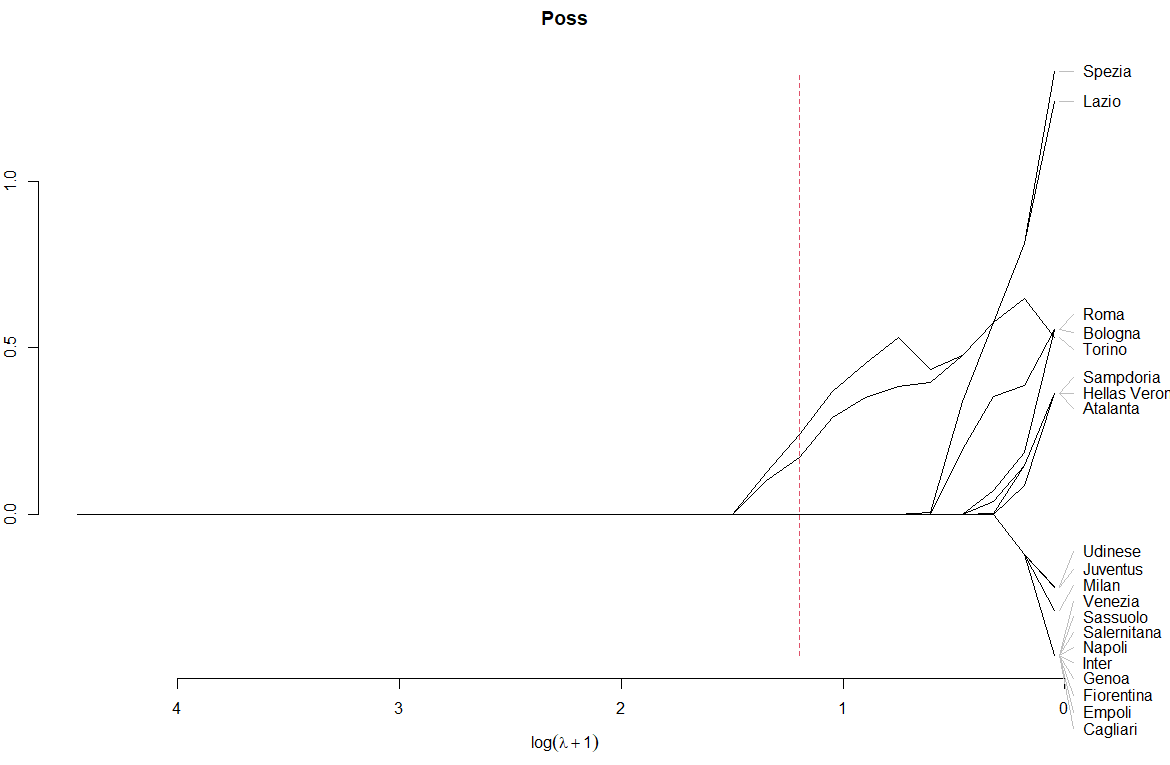
\includegraphics[height=8cm, width=15cm]{possL.png}
		\caption{Grafico che riporta l'andamento della stima del possesso della palla per ogni squadra al variare del parametro di tuning $\lambda$} \label{fig:possL}
	\end{center}
\end{figure}

In Figura \ref{fig:possL} viene mostrato l'andamento relativo alla stima della covariata del possesso della palla, in cui si notano la Lazio e il Torino che si discostano nettamente dall'andamento nullo tenuto dalla maggior parte delle squadre.

\begin{figure}[htbp]
	\begin{center}
		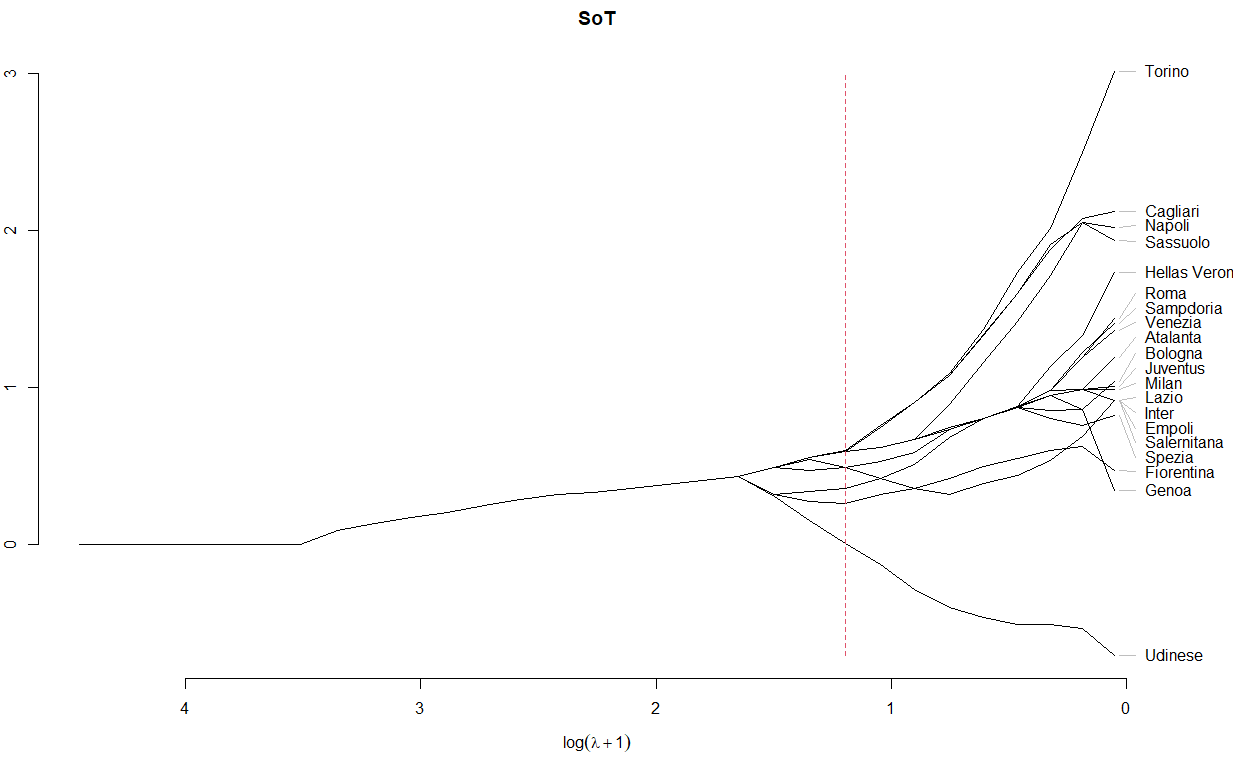
\includegraphics[height=8cm, width=15cm]{sotL.png}
		\caption{Grafico che riporta l'andamento della stima del numero di tiri in porta per ogni squadra al variare del parametro di tuning $\lambda$} \label{fig:sotL}
	\end{center}
\end{figure}

In Figura \ref{fig:sotL} viene mostrato l'andamento relativo alla stima della covariata del numero di tiri in porta. Si notano cinque clusters con stima positiva. Abbiamo il cluster con la stima più alta che contiene la maggioranza delle squadre, seguito dal secondo cluster per stima contenente Inter e Roma. Il terzo cluster per stima contiene solo il Bologna, anche il quarto cluster per stima contiene solo una squadra cioè la Fiorentina. Infine il quinto cluster per stima contiene l'Udinese che ha un valore quasi nullo ma comunque positivo.

\begin{figure}[htbp]
	\begin{center}
		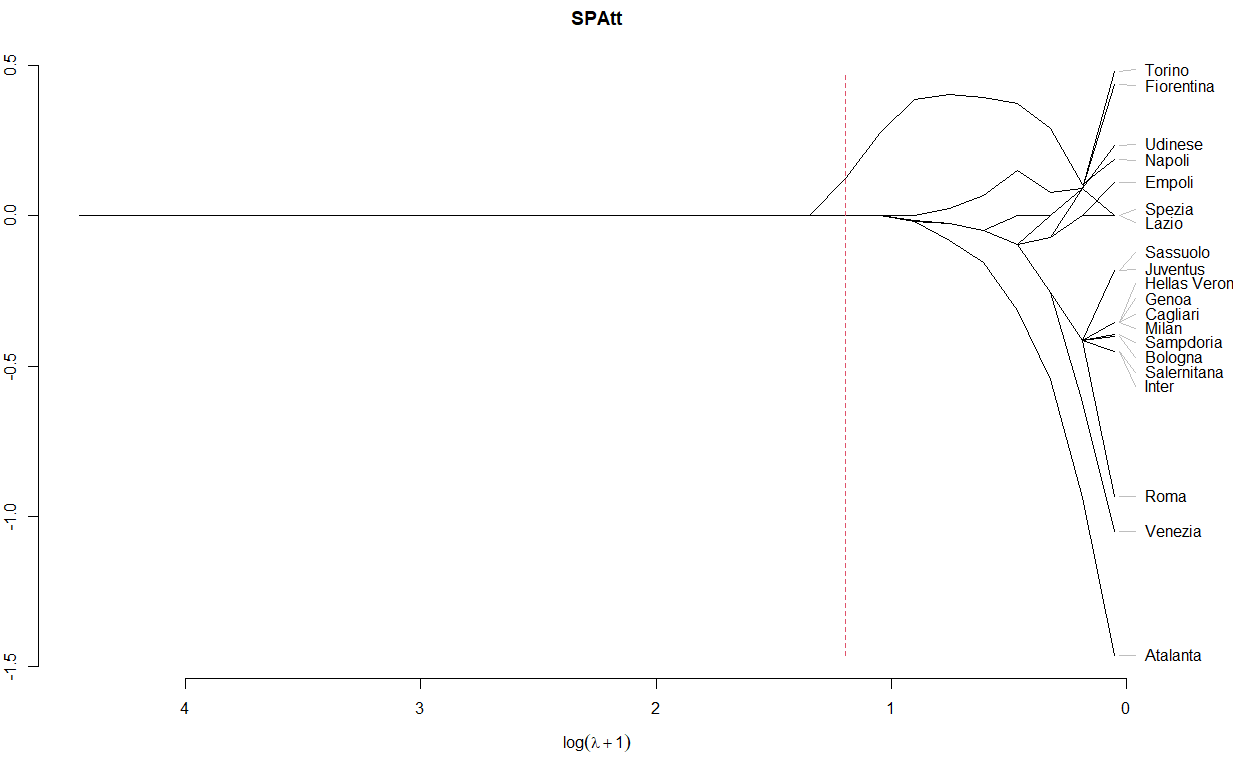
\includegraphics[height=8cm, width=15cm]{spattL.png}
		\caption{Grafico che riporta l'andamento della stima del numero di passaggi corti tentati per ogni squadra al variare del parametro di tuning $\lambda$} \label{fig:spattL}
	\end{center}
\end{figure}

In Figura \ref{fig:spattL} viene mostrato l'andamento relativo alla stima della covariata del numero di passaggi corti tentati. Si nota che il Napoli ha un andamento positivo che si discosta nettamente dall'andamento nullo tenuto dalla maggior parte delle squadre.

\begin{figure}[htbp]
	\begin{center}
		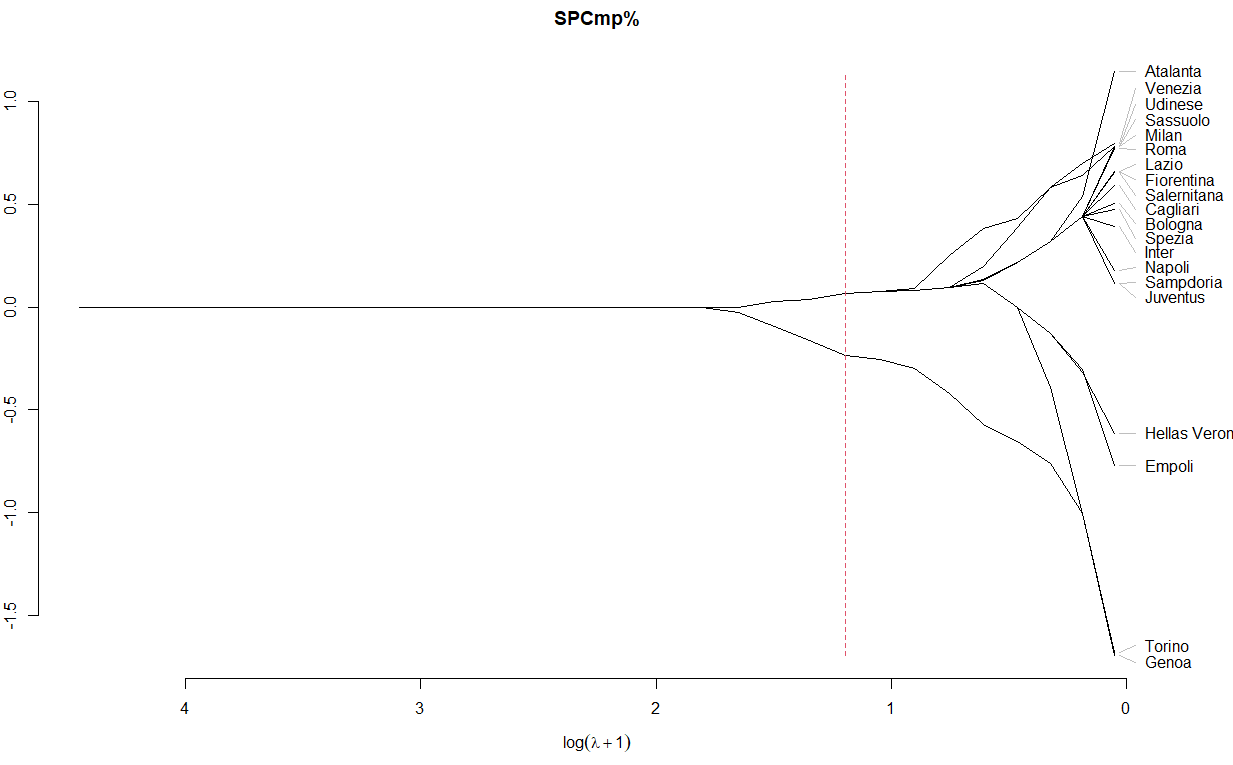
\includegraphics[height=8cm, width=15cm]{spcmpL.png}
		\caption{Grafico che riporta l'andamento della stima della percentuale di passaggi corti riusciti per ogni squadra al variare del parametro di tuning $\lambda$} \label{fig:spcmpL}
	\end{center}
\end{figure}

In Figura \ref{fig:spcmpL} viene mostrato l'andamento relativo alla stima della covariata della percentuale di passaggi corti riusciti. Si nota che il Genoa ha un andamento negativo che si discosta nettamente dall'andamento leggermente positivo tenuto dalla maggior parte delle squadre.

\begin{figure}[htbp]
	\begin{center}
		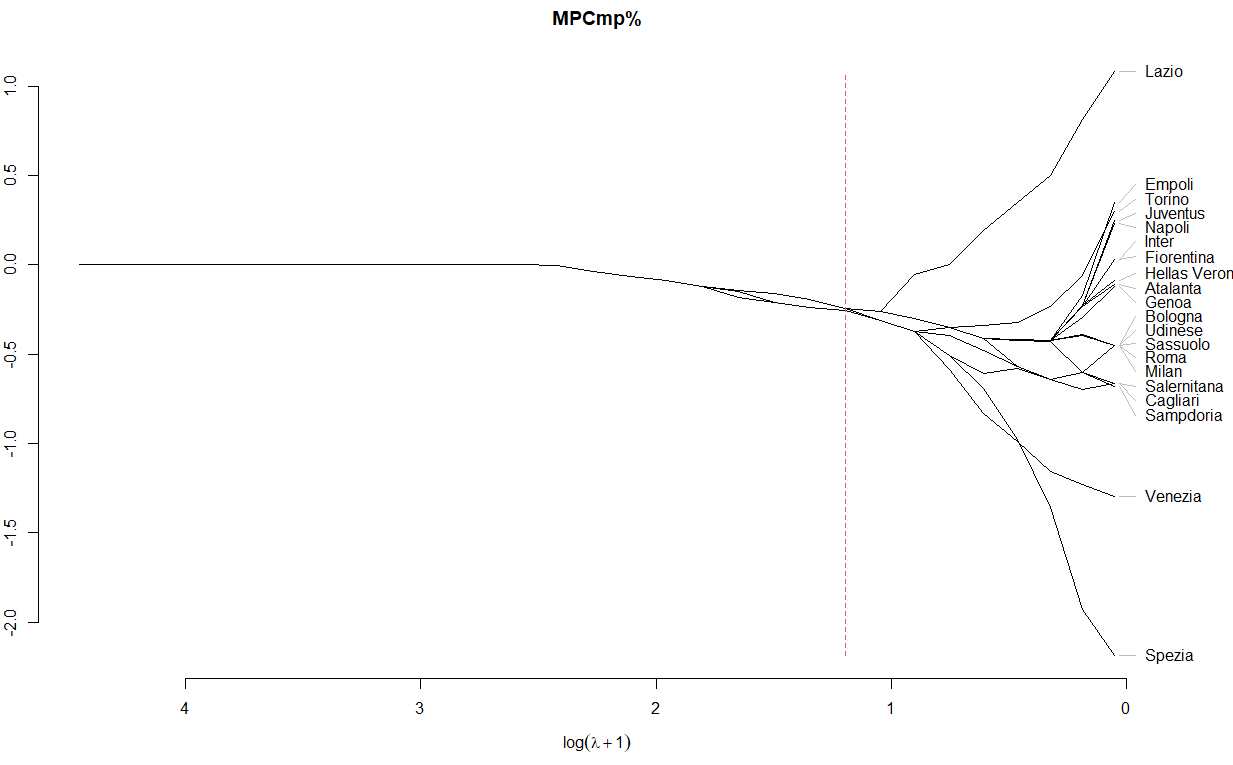
\includegraphics[height=8cm, width=15cm]{mpcmpL.png}
		\caption{Grafico che riporta l'andamento della stima della percentuale di passaggi medi riusciti per ogni squadra al variare del parametro di tuning $\lambda$} \label{fig:mpcmpL}
	\end{center}
\end{figure}

In Figura \ref{fig:mpcmpL} viene mostrato l'andamento relativo alla stima della covariata della percentuale di passaggi medi riusciti. Si nota che il Genoa e il Bologna hanno un andamento leggermente più negativo rispetto all'andamento comunque negativo tenuto dalla maggior parte delle squadre.

\begin{figure}[htbp]
	\begin{center}
		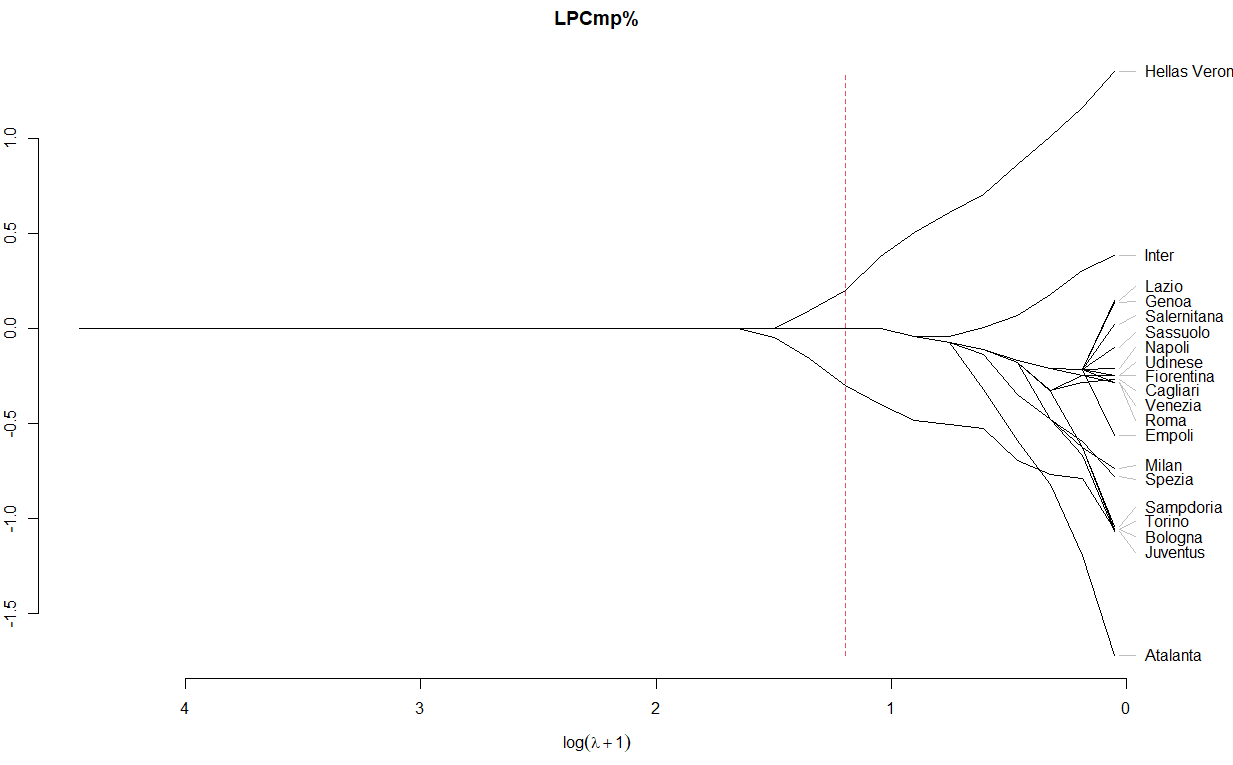
\includegraphics[height=8cm, width=15cm]{lpcmpL.png}
		\caption{Grafico che riporta l'andamento della stima della percentuale di passaggi lunghi riusciti per ogni squadra al variare del parametro di tuning $\lambda$} \label{fig:lpcmpL}
	\end{center}
\end{figure}

In Figura \ref{fig:lpcmpL} viene mostrato l'andamento relativo alla stima della covariata della percentuale di passaggi lunghi riusciti. Ci sono tre clusters. C'è il cluster contenete l'Hellas Verona che ha un percorso positivo, il cluster più grande che contiene quasi tutte le squadre ha un andamento nullo e Infine, il terzo cluster contenete il Bologna ha un andamento negativo.

\begin{figure}[htbp]
	\begin{center}
		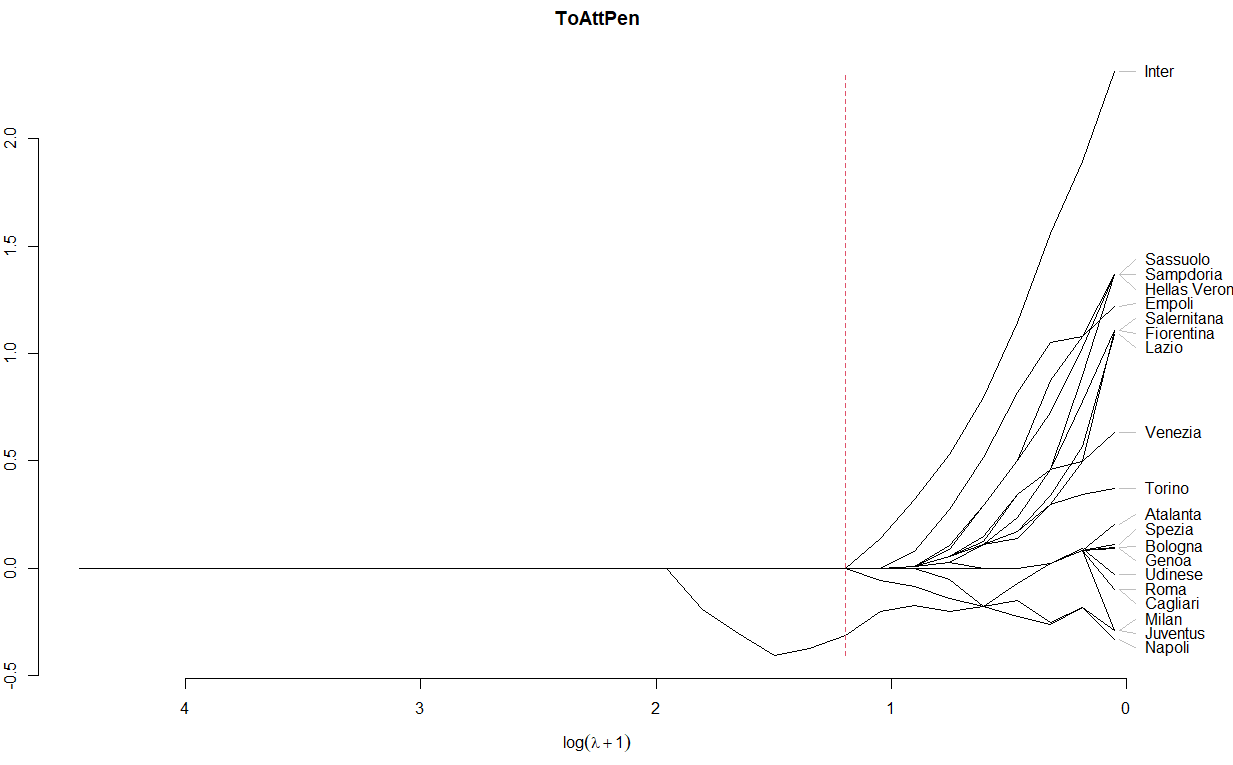
\includegraphics[height=8cm, width=15cm]{toattpenL.png}
		\caption{Grafico che riporta l'andamento della stima del numero di tocchi fatti nell'area di rigore avversaria per ogni squadra al variare del parametro di tuning $\lambda$} \label{fig:toattpenL}
	\end{center}
\end{figure}

In Figura \ref{fig:toattpenL} viene mostrato l'andamento relativo alla stima della covariata del numero di tocchi fatti nell'area di rigore avversari. Si nota che l'Atalanta ha un andamento negativo che si discosta nettamente dall'andamento nullo tenuto dalla maggior parte delle squadre.

\begin{figure}[htbp]
	\begin{center}
		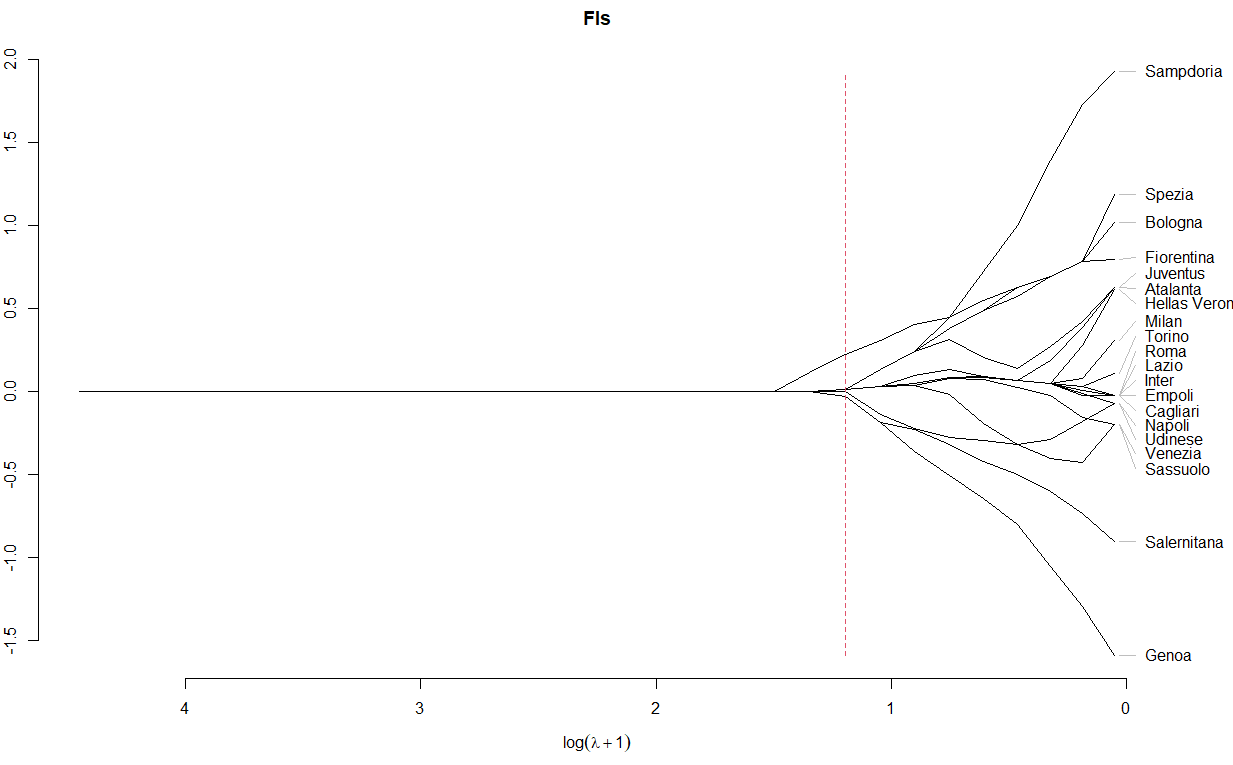
\includegraphics[height=8cm, width=15cm]{flsL.png}
		\caption{Grafico che riporta l'andamento della stima del numero di falli subiti per ogni squadra al variare del parametro di tuning $\lambda$} \label{fig:flsL}
	\end{center}
\end{figure}

In Figura \ref{fig:flsL} viene mostrato l'andamento relativo alla stima della covariata del numero di falli subiti, in cui si notano quattro clusters. C'è il cluster contenete il Bologna che ha un percorso positivo, il cluster più grande che contiene quasi tutte le squadre che ha un andamento leggermente positivo. Invece il cluster che contiene il Napoli ha un andamento leggermente negativo, mentre ancora più negativo è il cluster contente il Genoa e la Salernitana.

\begin{figure}[htbp]
	\begin{center}
		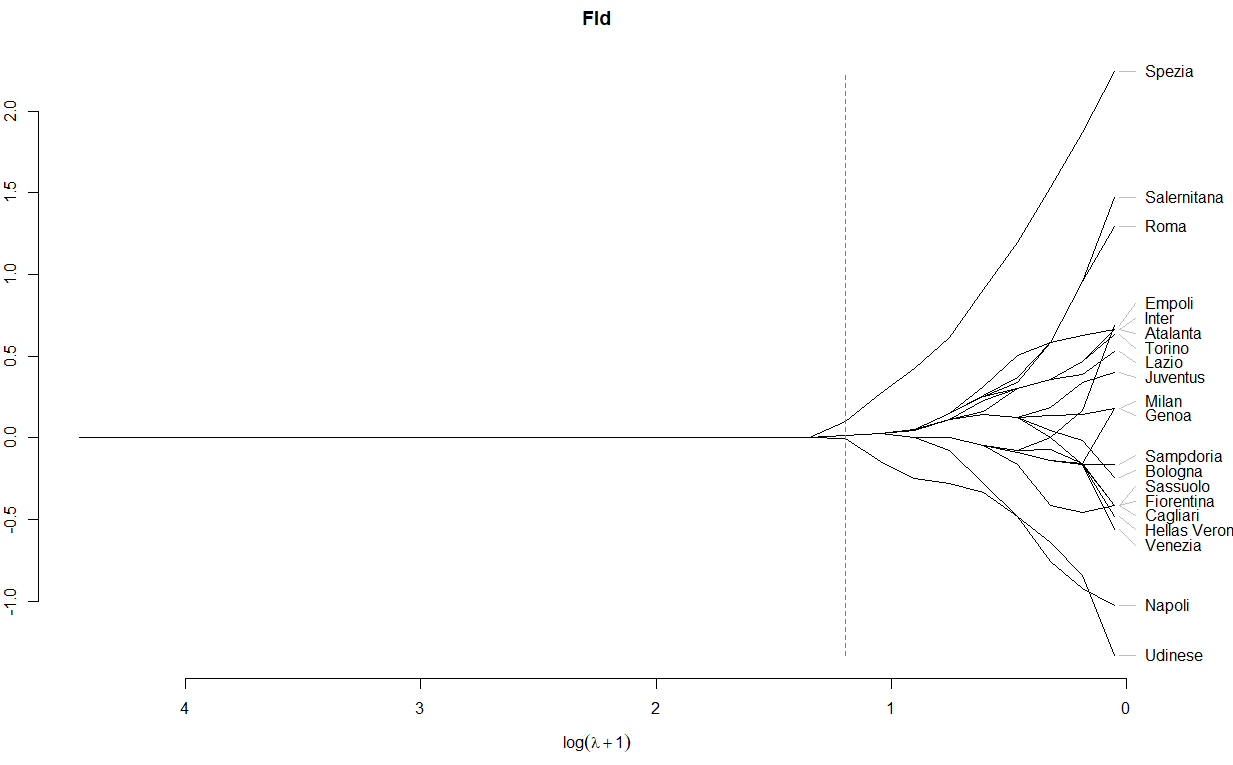
\includegraphics[height=8cm, width=15cm]{fldL.png}
		\caption{Grafico che riporta l'andamento della stima del numero di falli fatti per ogni squadra al variare del parametro di tuning $\lambda$} \label{fig:fldL}
	\end{center}
\end{figure}

In Figura \ref{fig:fldL} viene mostrato l'andamento relativo alla stima della covariata del numero di falli fatti, in cui si notano tre clusters. C'è il cluster contenete lo Spezia che ha un percorso positivo, il cluster più grande che contiene quasi tutte le squadre che ha un andamento leggermente positivo. Invece il cluster che contiene l'Udinese ha un andamento leggermente negativo.

\begin{figure}[htbp]
	\begin{center}
		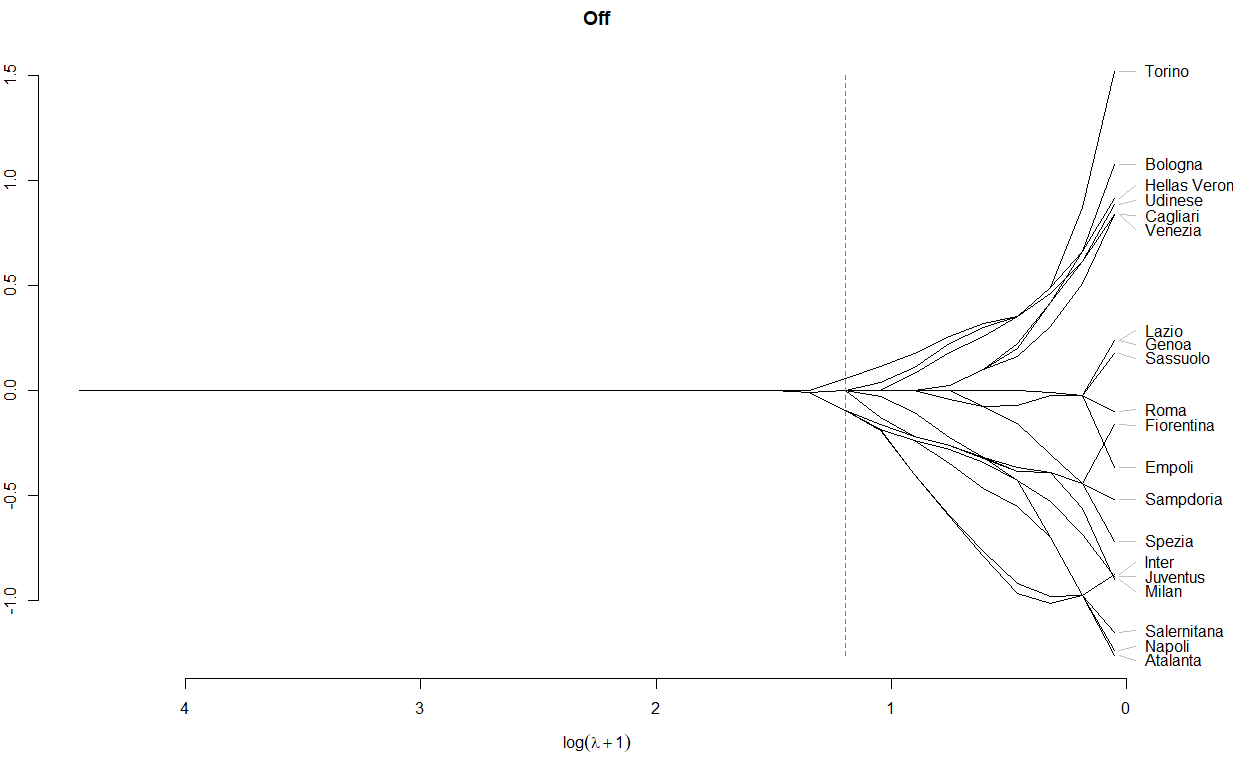
\includegraphics[height=8cm, width=15cm]{offL.png}
		\caption{Grafico che riporta l'andamento della stima del numero di fuorigioco fatti per ogni squadra al variare del parametro di tuning $\lambda$} \label{fig:offL}
	\end{center}
\end{figure}

In Figura \ref{fig:offL} viene mostrato l'andamento relativo alla stima della covariata del numero di fuorigioco fatti. Ci sono tre clusters. C'è il cluster contenete l'Hellas Verona che ha un percorso positivo, il cluster più grande che contiene quasi tutte le squadre che ha un andamento leggermente positivo. Infine c'è il cluster che contiene il Milan, l'Inter, il Napoli e la Juventus che ha un andamento negativo.

\begin{figure}[htbp]
	\begin{center}
		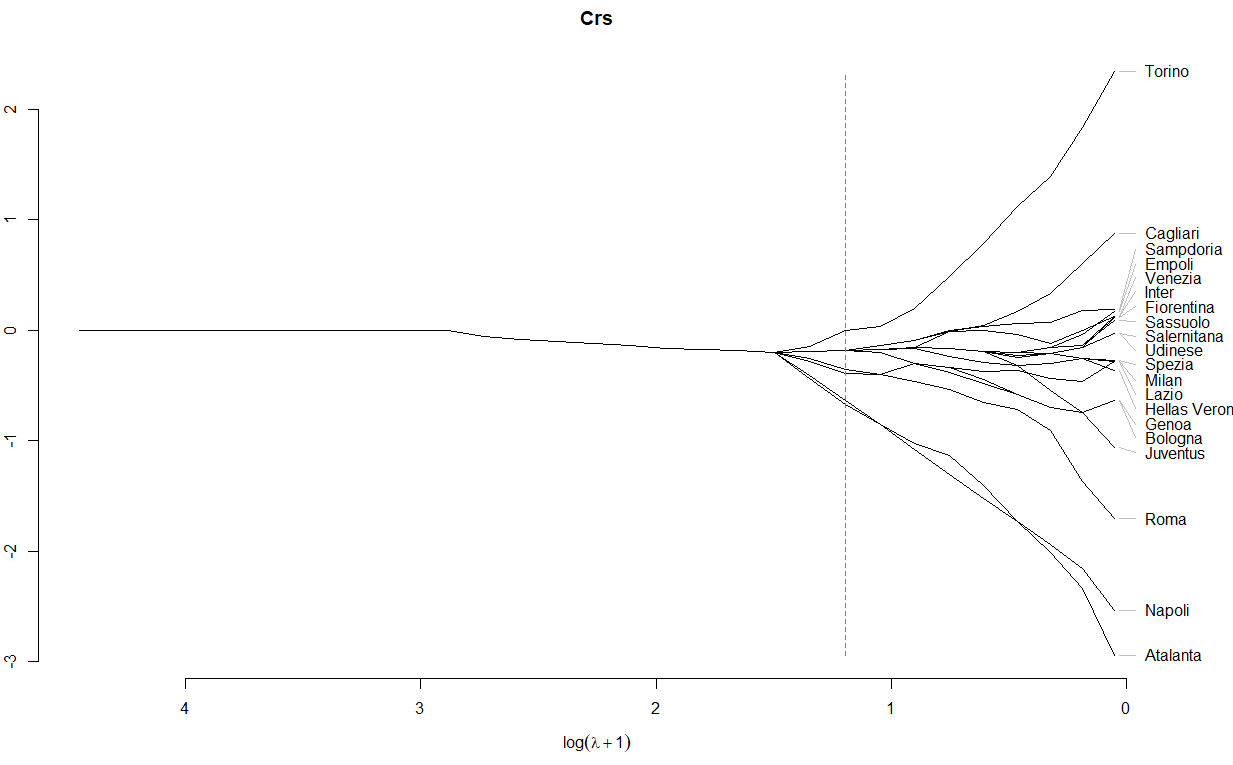
\includegraphics[height=8cm, width=15cm]{crsL.png}
		\caption{Grafico che riporta l'andamento della stima del numero di cross fatti per ogni squadra al variare del parametro di tuning $\lambda$} \label{fig:crsL}
	\end{center}
\end{figure}

In Figura \ref{fig:crsL} viene mostrato l'andamento relativo alla stima della covariata del numero di cross fatti. Ci sono quattro clusters. C'è il cluster contenete il Torino che ha un andamento nullo, il cluster più grande che contiene quasi tutte le squadre che ha un percorso negativo. Ancora più negativi sono i percorsi del cluster contenente il Milan e la Roma, secondo solo al cluster contenente l'Atalanta e il Napoli che si discosta nettamente da tutti gli altri clusters.

\begin{figure}[htbp]
	\begin{center}
		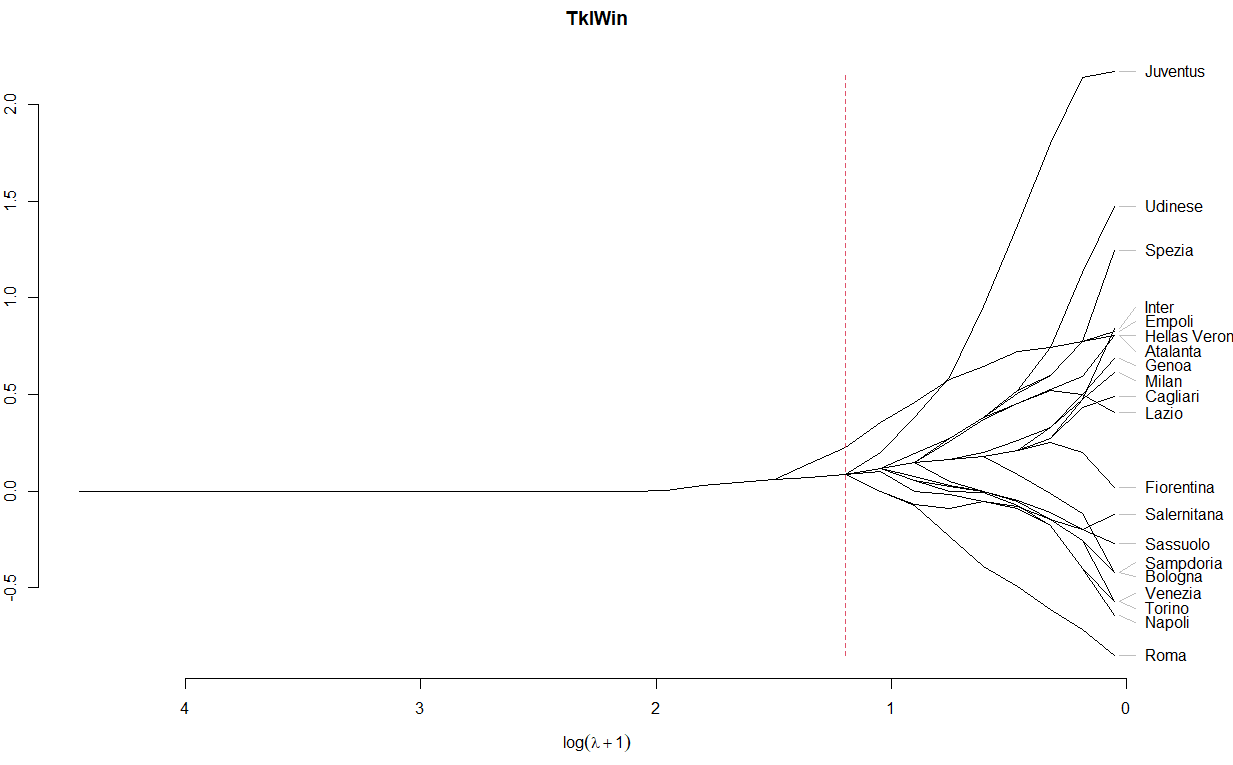
\includegraphics[height=8cm, width=15cm]{tklwinL.png}
		\caption{Grafico che riporta l'andamento della stima del numero di contrasti vinti per ogni squadra al variare del parametro di tuning $\lambda$} \label{fig:tklwinL}
	\end{center}
\end{figure}

\begin{figure}[htbp]
	\begin{center}
		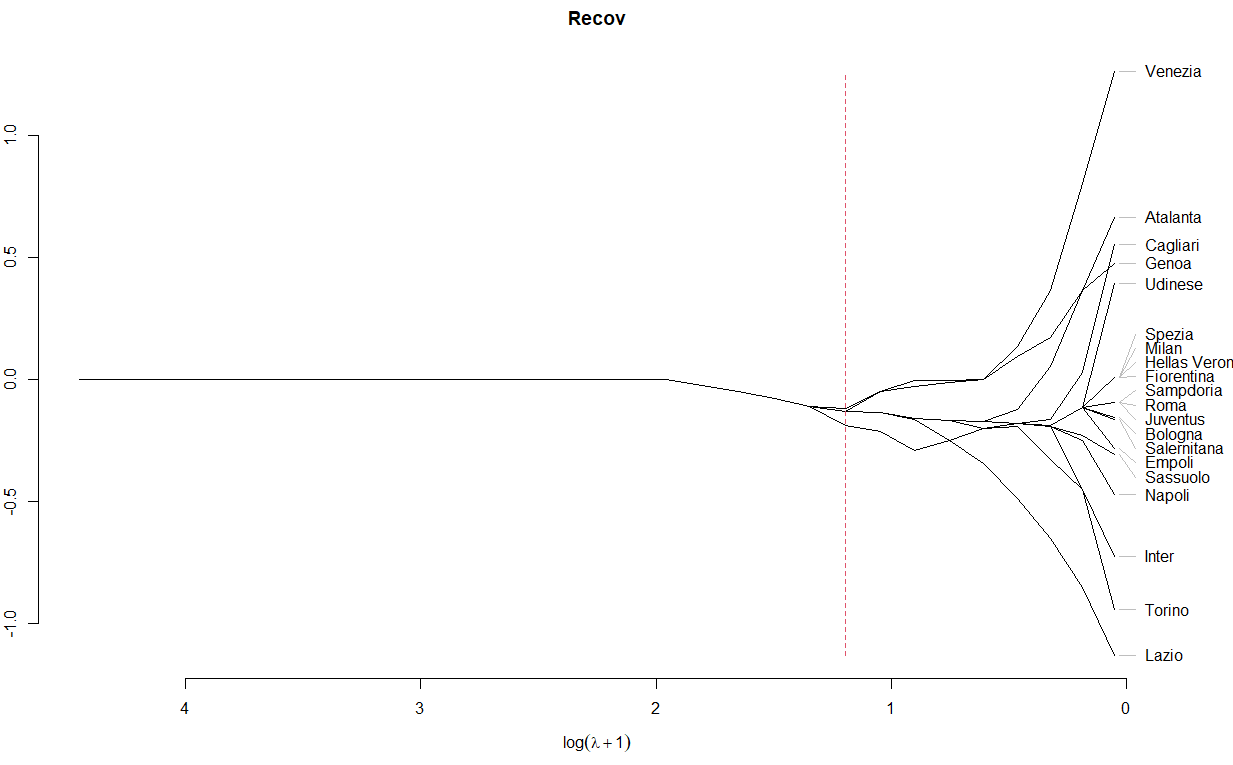
\includegraphics[height=8cm, width=15cm]{recovL.png}
		\caption{Grafico che riporta l'andamento della stima del numero di recuperi per ogni squadra al variare del parametro di tuning $\lambda$} \label{fig:recovL}
	\end{center}
\end{figure}
In Figura \ref{fig:tklwinL} viene mostrato l'andamento relativo alla stima della covariata del numero di contrasti vinti, in cui si nota che l'Empoli ha un percorso positivo che si discosta nettamente dall'andamento comunque positivo ma in minor misura, tenuto dalla maggior parte delle squadre.\\
In Figura \ref{fig:recovL} viene mostrato l'andamento relativo alla stima della covariata del numero di recuperi. Si nota che l'Udinese ha un percorso leggermente più negativo rispetto all'andamento negativo tenuto dalla maggior parte delle squadre.\\

Per riassumere quanto visto fin ora, la Figura \ref{fig:l2BTCL} mostra i percorsi delle norme L2 che rappresentano l'importanza complessiva dei singoli effetti delle covariate.

\begin{figure}[htbp]
	\begin{center}
		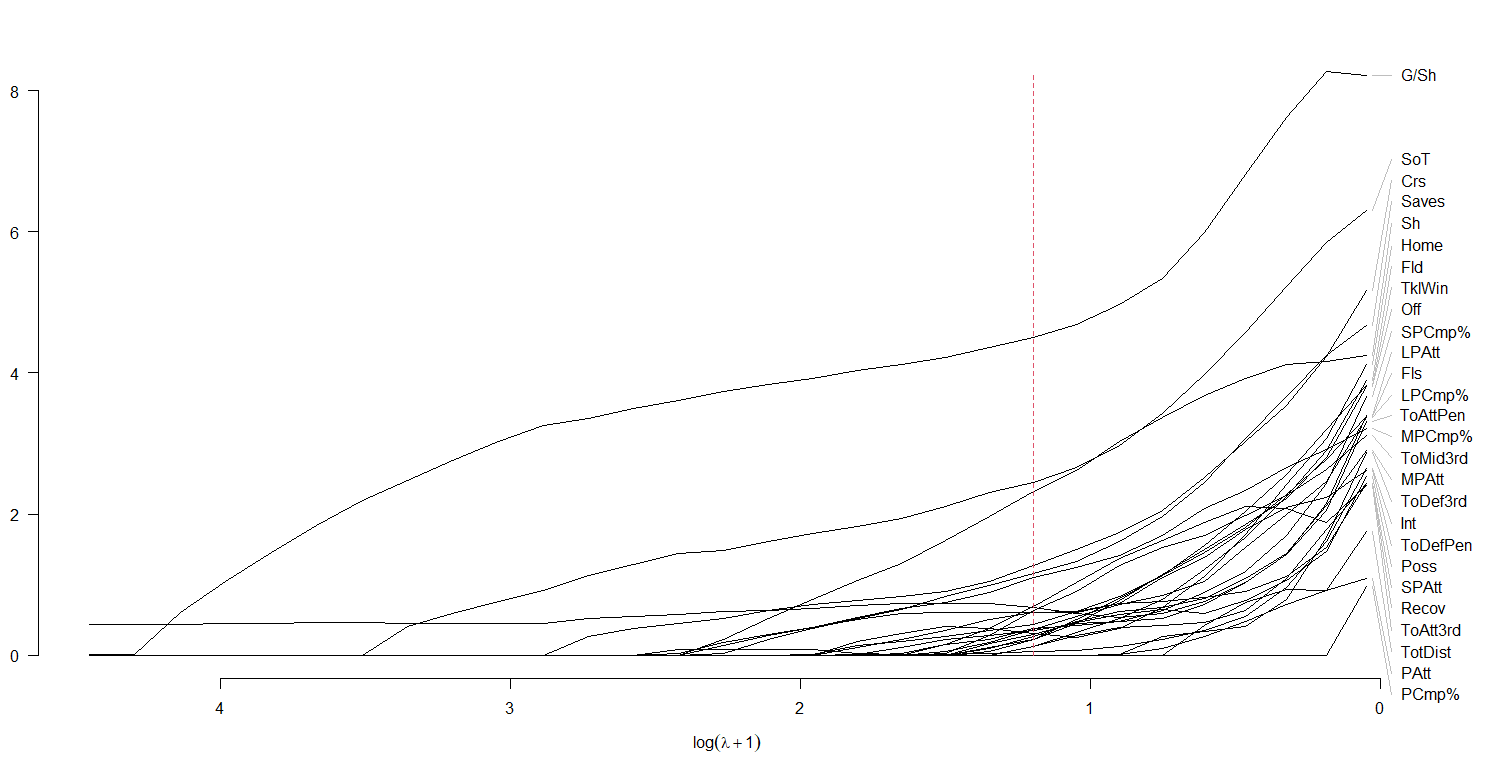
\includegraphics[height=8cm, width=15cm]{L2.png}
		\caption{Grafico che riporta l'importanza delle covariate rispetto alle norme L2 al variare del parametro di tuning $\lambda$} \label{fig:l2BTCL}
	\end{center}
\end{figure}
Dal grafico si nota che il rapporto tiri-gol \texttt{G/Sh} è la variabile che incide maggiormente nella determinazione dell'esito di una partita. Analogamente anche il numero di tiri in porta \texttt{SoT} e il numero di parate \texttt{Saves} sono determinanti dell'esito di una partita, ma con un minor peso rispetto a \texttt{G/Sh}. Anche il numero di cross \texttt{Crs} determina in modo significativo l'esito della partita, ma al contrario di \texttt{G/Sh} sappiamo che contribuisce a diminuire le probabilità di vittoria. Si nota anche qui che il possesso della palla ha un ruolo molto marginale nel determinare il risultato di una partita. Viene confermata la tendenza che mantenere il pallone in zone difensive con meno transizioni in zone d'attacco sembra che dia maggior probabilità di vittoria. Si riconferma il numero di lanci lunghi tentati \texttt{LPAtt} importante per l'esito della partita e che favorisce la vittoria. Al contrario le altre variabili esplicative legate ai passaggi che sono poco determinanti e diminuiscono la probabilità di vittoria. Dal grafico si nota che sia il numero di contrasti vinti \texttt{TklWin} e il numero di fuorigioco \texttt{Off} sono determinanti, diversamente il numero di recuperi \texttt{Recov}, la distanza percorsa con la palla \texttt{TotDist} e il numero di intercetti \texttt{Int} sono poco significativi. Infine notiamo che il numero di falli fatti \texttt{fld} è più determinante di quelli subiti \texttt{fls}.\\
Perciò, la maggior parte delle stime ottenute sembrano essere in linea con i risultati osservati nel precedente modello con covariate specifiche dell'oggetto senza l'applicazione del metodo \emph{LASSO}.

\section{BTM senza l'intercetta e con LASSO}
Come era stato accennato nel Capitolo \ref{cap:BT} l'intercetta spiega la maggior parte dell'abilità relativa alla squadra. Per cui le covariate possono essere viste come estensioni contenenti effetti aggiuntivi dell'abilità della squadra che non sono spiegati dall'intercetta. In tal senso, gli effetti della covariata possono aiutare a spiegare i risultati imprevisti di un partita che non possono essere completamente spiegati esclusivamente dall'intercetta. Nelle tre precedenti applicazione del modello Bradley-Terry si è sempre inserita un intercetta per ogni squadra, anche nel modello \hyperref[for:3.9]{(4.9)}. Perciò, di seguito verranno mostrati i risultati relativi a un modello Bradley-Terry della stessa forma del modello \hyperref[for:4.9]{(4.12)} ma senza le intercette, con lo scopo di capire qual'è l'effetto totale che ha ogni variabile esplicativa sull'abilità della squadra senza l'interferenza dell'intercetta che copre l'effetto della covariata. Ovviamente dato il numero elevato di covariate è stata applicata una selezione attraverso il metodo \emph{LASSO}. Il modello applicato è il seguente
\begin{align}
	P(Y_{p(i,j)}\leq k) =  \frac{exp(\delta_i + \theta_{k} + x^T_{pi}\eta_i - x^T_{pj}\eta_j)}{1 + exp(\delta_i + \theta_{k} + x^T_{pi}\eta_i - x^T_{pj}\eta_j)},\label{for:5.2}
\end{align}

Nella Tabella \ref{tab:BTCLI2} e nella Tabella \ref{tab:BTCLI3} vengono riportati i risultati nella stessa modalità utilizza nella precedente sezione.
\begin{table}[]%
	
	\renewcommand{\arraystretch}{1.7}
	\centering
	\begin{tabular}{ccp{10cm}}
		\hline	
		
		\textbf{Covariata} & \textbf{Stima} & \textbf{Squadra} \\	
		\hline
		Home & 0.270 & Tutti\\
		Poss & 0.299 & Lazio \\
		Poss & 0.047 & Tutti tranne Lazio\\
		Sh & 0.317 & Tutti \\
		SoT & 0.495 & Atalanta, Cagliari, Empoli, Genoa, Verona, Juventus, Lazio, Milan, Napoli, Roma, Salernitana, Sampdoria, Sassuolo, Spezia, Torino e Venezia\\
		SoT & 0.438 & Inter\\
		SoT & 0.399 & Bologna, Fiorentina e Udinese \\
		G/Sh & 0.867 & Tutti \\
		Saves & 0.242 & Tutti \\
		PAtt & 0.000 & Tutti \\
		PCmp\% & 0.000 & Tutti \\
		SPAtt & 0.000 & Tutti \\
		SPCmp\% & 0.000 & Tutti tranne Genoa \\ 
		SPCmp\% & -0.076 & Genoa \\	
		MPAtt & 0.000 & Tutti \\ 
		MPCmp\% & -0.230 & Udinese \\
		MPCmp\% & -0.236 & Tutti tranne Udinese \\		
		LPAtt & 0.178 & Tutti \\
		LPCmp\% & 0.016 & Hellas Verona \\
		LPCmp\% & 0.000 & Tutti tranne Verona \\
		ToDefPen & 0.080 & Tutti \\      
		ToDef3rd & 0.024 & Tutti \\
		
		
		\hline
		& &  \\
		
	\end{tabular} \hbox{}
	\caption{Stime delle covariate.} \label{tab:BTCLI2} 
	
\end{table}

\begin{table}[]%
	
	\renewcommand{\arraystretch}{1.7}
	\centering
	\begin{tabular}{ccp{10cm}}
		\hline	
		
		\textbf{Covariata} & \textbf{Stima} & \textbf{Squadra} \\	
		\hline
		ToMid3rd & 0.002 & Tutti tranne Inter e Sampdoria\\
		ToMid3rd & 0.000 & Inter e Sampdoria\\
		ToAtt3rd & -0.013 & Tutti \\  
		ToAttPen & 0.035 & Tutti tranne Atalanta \\    
		ToAttPen & -0.083 & Atalanta \\ 	     	 
		TotDist & 0.000 & Tutti \\	
		Fls & 0.256 & Bologna  \\
		Fls & 0.088 & Tutti tranne Bologna \\ 		
		Fld & 0.066 & Tutti tranne Udinese \\
		Fld & 0.023 & Udinese \\
		Off & 0.055 & Hellas Verona\\
		Off & 0.000 & Tutti tranne Juventus\\
		Off & -0.085 & Juventus  \\
		Crs & -0.190 & Tutti tranne Atalanta\\
		Crs & -0.464 & Atalanta \\
		Int & 0.000 & Tutti\\
		TklWin &  0.117 & Empoli  \\
		TklWin &  0.000 & Tutti tranne Empoli  \\ 
		Recov &  0.000 & Tutti \\ 
		\hline
		& &  \\
		
	\end{tabular} \hbox{}
	\caption{Stime delle covariate.} \label{tab:BTCLI3} 
	
\end{table}
Anche in questa applicazione sono state eliminate alcune covariate. Come già visto nel modello precedente, vengono confermate l'eliminazione del numero di passaggi tentati \texttt{PAtt}, della percentuale dei passaggi completati \texttt{PCmp\%} e della distanza percorsa con la palla \texttt{TotDist}. Viene tolta dal modello la variabile esplicativa del numero di passaggi corti tentati \texttt{SPAtt} che nel modello precedente andava a aumentare le probabilità di vittoria solo per il Napoli. Viene eliminata la covariata del numero di passaggi medi tentati \texttt{MPAtt} e quella del numero di intercettazioni \texttt{Int}. Infine abbiamo l'eliminazione della variabile esplicativa che indica il numero di recuperi che nel precedente modello era valutata come una covariata che incideva negativamente sulla probabilità di vittoria.\\

In questa nuovo tipo di modello la stima del parametro del possesso palla \texttt{Poss} ha subito un piccola variazione. Infatti ora la stima non è più nulla per la maggior parte delle squadre ma e leggermente positiva. Ciononostante la significatività si riconferma ancora bassa. Si riconferma però significativa solo per il gioco della Lazio ma non più per il Torino come nello scorso modello. Tale risultato è visibili nella Figura \ref{fig:possLI}.\\
\begin{figure}[]
	\begin{center}
		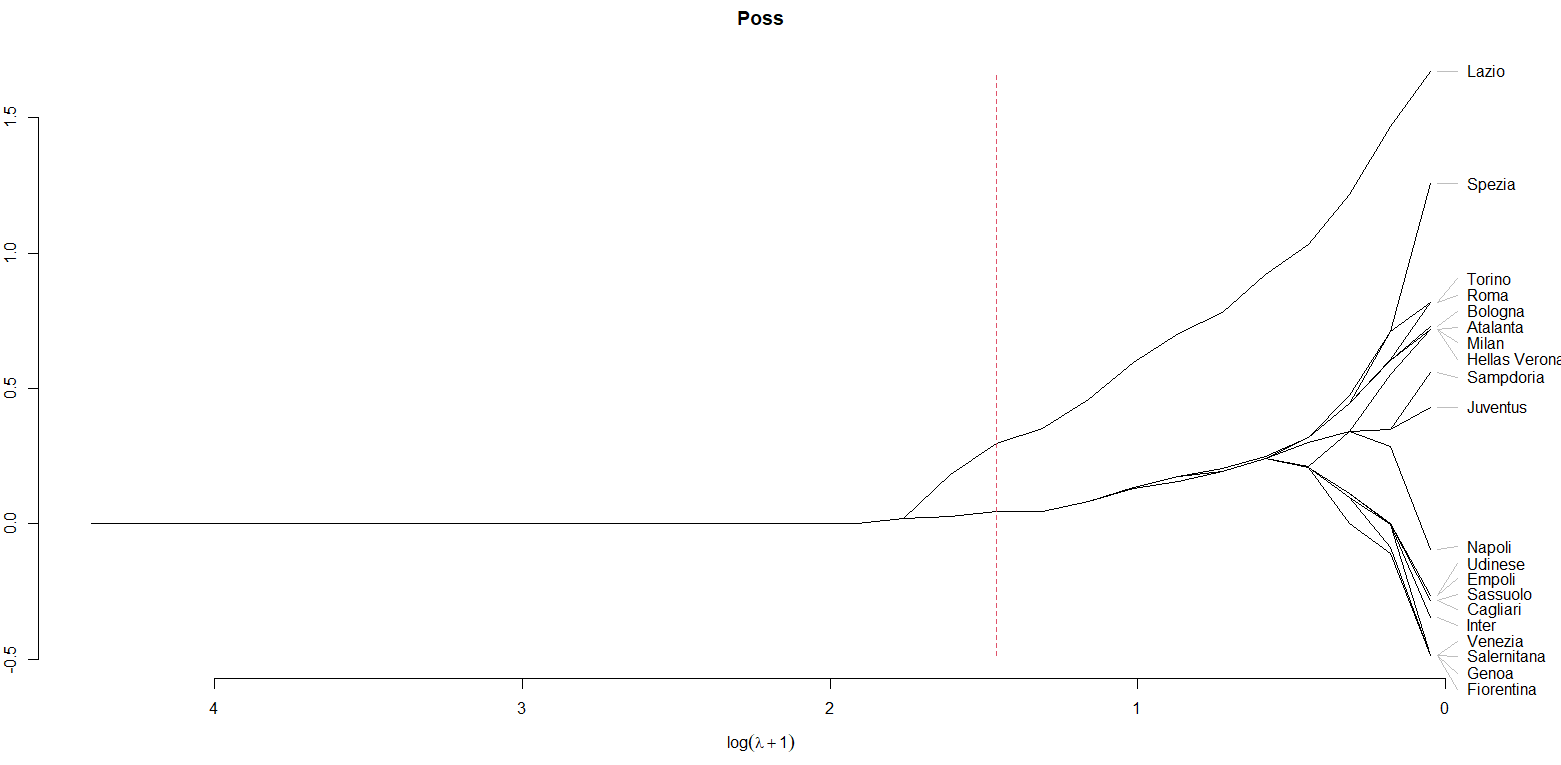
\includegraphics[height=8cm, width=15cm]{possLI.png}
		\caption{Grafico che riporta l'andamento della stima del possesso della palla per ogni squadra al variare del parametro di tuning $\lambda$} \label{fig:possLI}
	\end{center}
\end{figure}
Il numero di tiri \texttt{Sh}, il rapporto tiri-gol \texttt{G/Sh} e il numero di parate \texttt{Saves} sono ancora determinati per aumentare la probabilità di vittoria. Analogamente anche il numero di tiri in porta \texttt{SoT} mantiene sia una stima positiva del parametro, e sia la sua variabilità seppur più ristretta rispetto al modello precedente. Infatti nella Figura \ref{fig:sotLI} è possibile individuare tre clusters. Il più grande con la maggiore stima contiene la maggior parte delle squadre. Il secondo contiene solo l'Inter e infine il terzo contiene le squadre: Bologna, Fiorentina e Udinese. Il risultato è visibile nella Figura \ref{fig:sotLI} \\
\begin{figure}[htbp]
	\begin{center}
		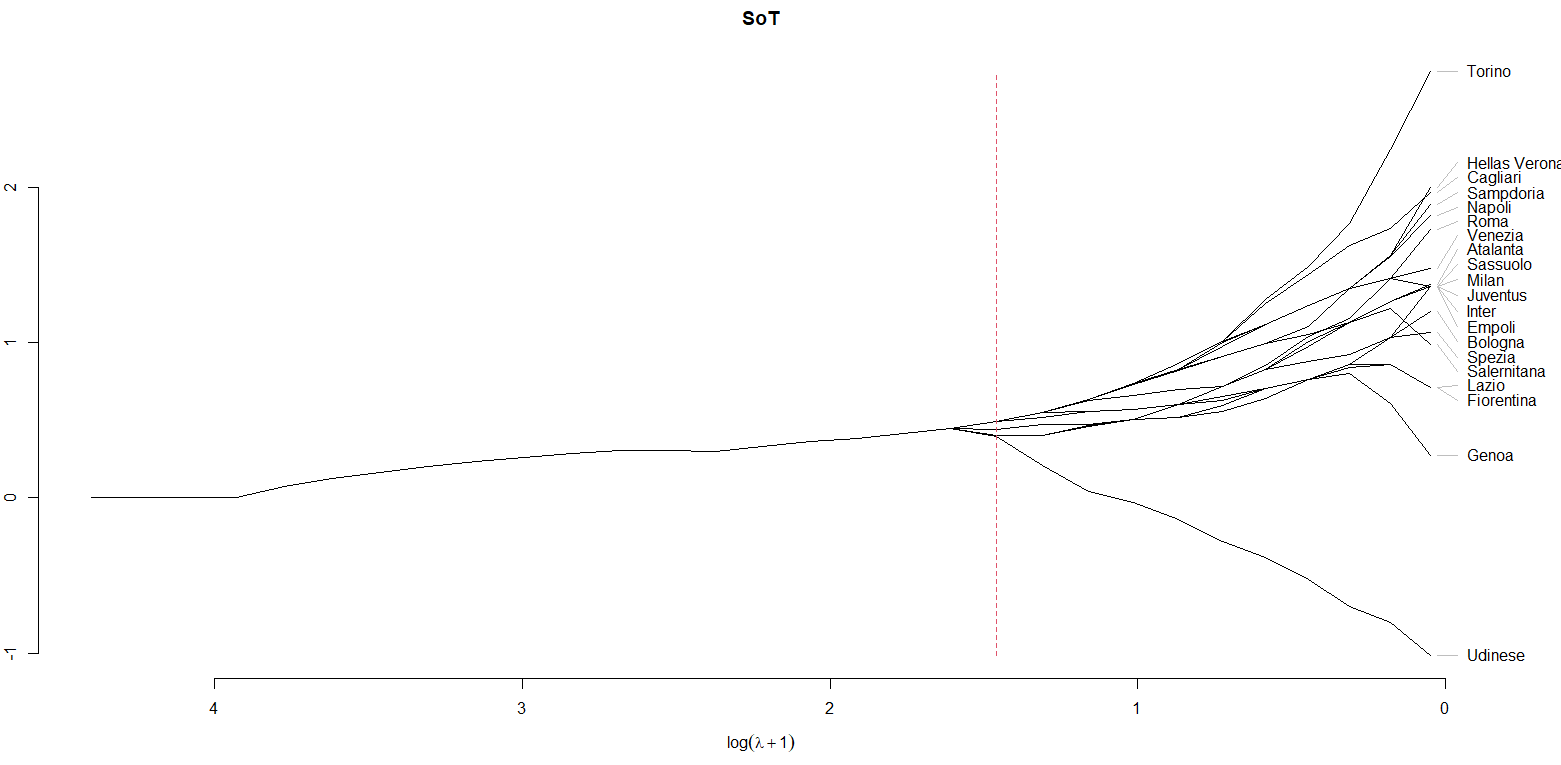
\includegraphics[height=8cm, width=15cm]{sotLI.png}
		\caption{Grafico che riporta l'andamento della stima del numero di tiri in porta per ogni squadra al variare del parametro di tuning $\lambda$} \label{fig:sotLI}
	\end{center}
\end{figure}
Nella percentuale di passaggi corti riusciti \texttt{SPCmp\%} ora viene a crearsi un cluster con un percorso nullo contenente quasi tutte le squadre eccetto il Genoa che è contenuto in un cluster con un percorso negativo. Tali risultati sono visibili nella Figura \ref{fig:spcmpLI}.\\
\begin{figure}[htbp]
	\begin{center}
		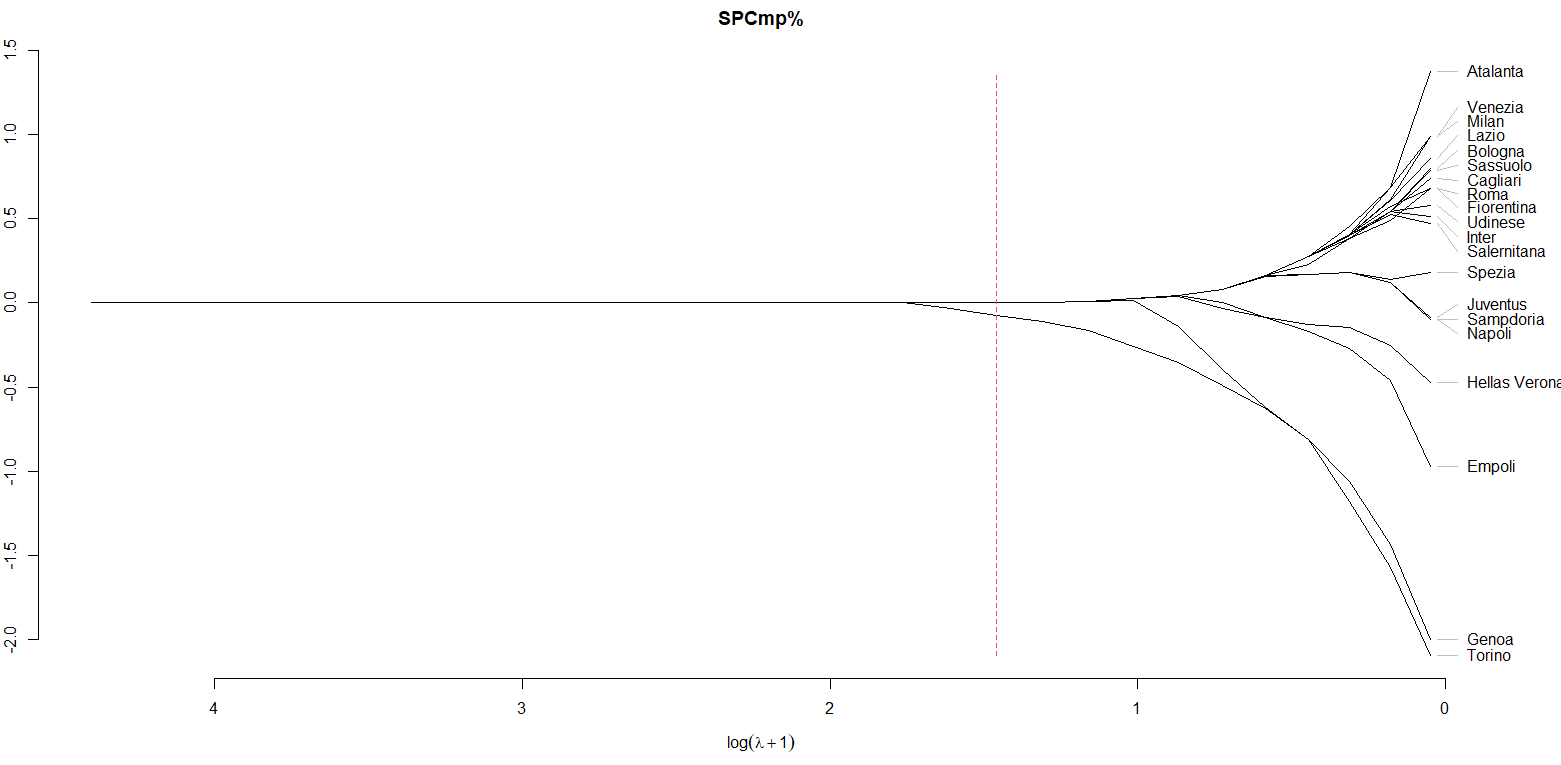
\includegraphics[height=8cm, width=15cm]{spcmpLI.png}
		\caption{Grafico che riporta l'andamento della stima della percentuale di passaggi corti riusciti per ogni squadra al variare del parametro di tuning $\lambda$} \label{fig:spcmpLI}
	\end{center}
\end{figure}
Per la variabile esplicativa della percentuale di passaggi medi riusciti \texttt{MPCmp\%} ora viene a crearsi un cluster con un percorso fortemente negativo contenente quasi tutte le squadre eccetto l'Udinese dove si distingue per avere un percorso leggermente meno negativo. Tali risultati sono visibili nella Figura \ref{fig:mpcmpLI}.\\
\begin{figure}[]
	\begin{center}
		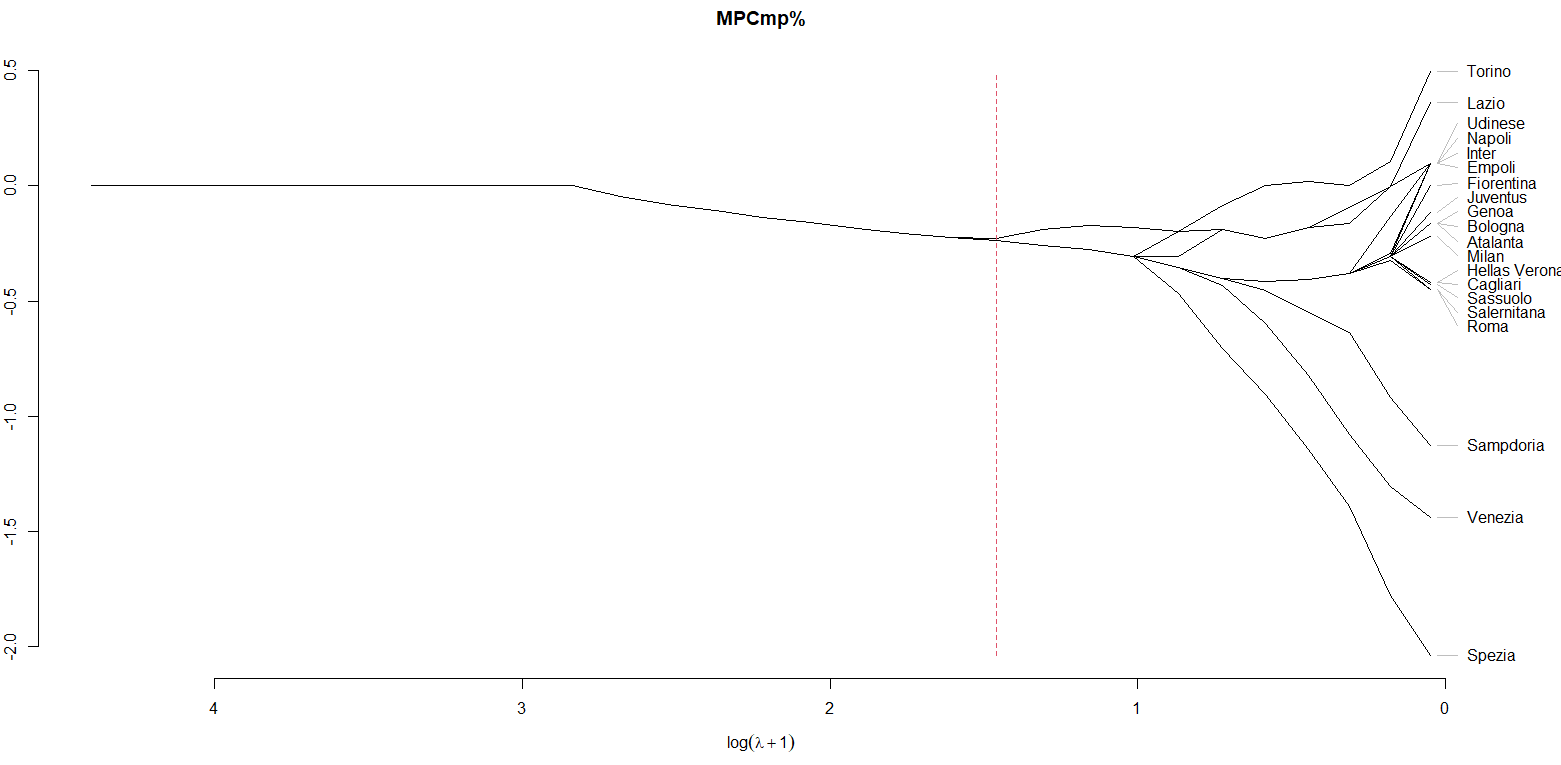
\includegraphics[height=8cm, width=15cm]{mpcmpLI.png}
		\caption{Grafico che riporta l'andamento della stima della percentuale di passaggi medi riusciti per ogni squadra al variare del parametro di tuning $\lambda$} \label{fig:mpcmpLI}
	\end{center}
\end{figure}
Il numero di passaggi lunghi tentati è ancora una covariata con una stima del parametro che aumenta la probabilità di vittoria. Si nota che la stima della covariata della percentuale di passaggi lunghi riusciti \texttt{LPCmp\%} ha un cluster con un percorso nullo contenente quasi tutte le squadre eccetto l'Hellas Verona che si distingue con un percorso positivo. Tali risultati sono visibili nella Figura \ref{fig:lpcmpLI}.\\
\begin{figure}[htbp]
	\begin{center}
		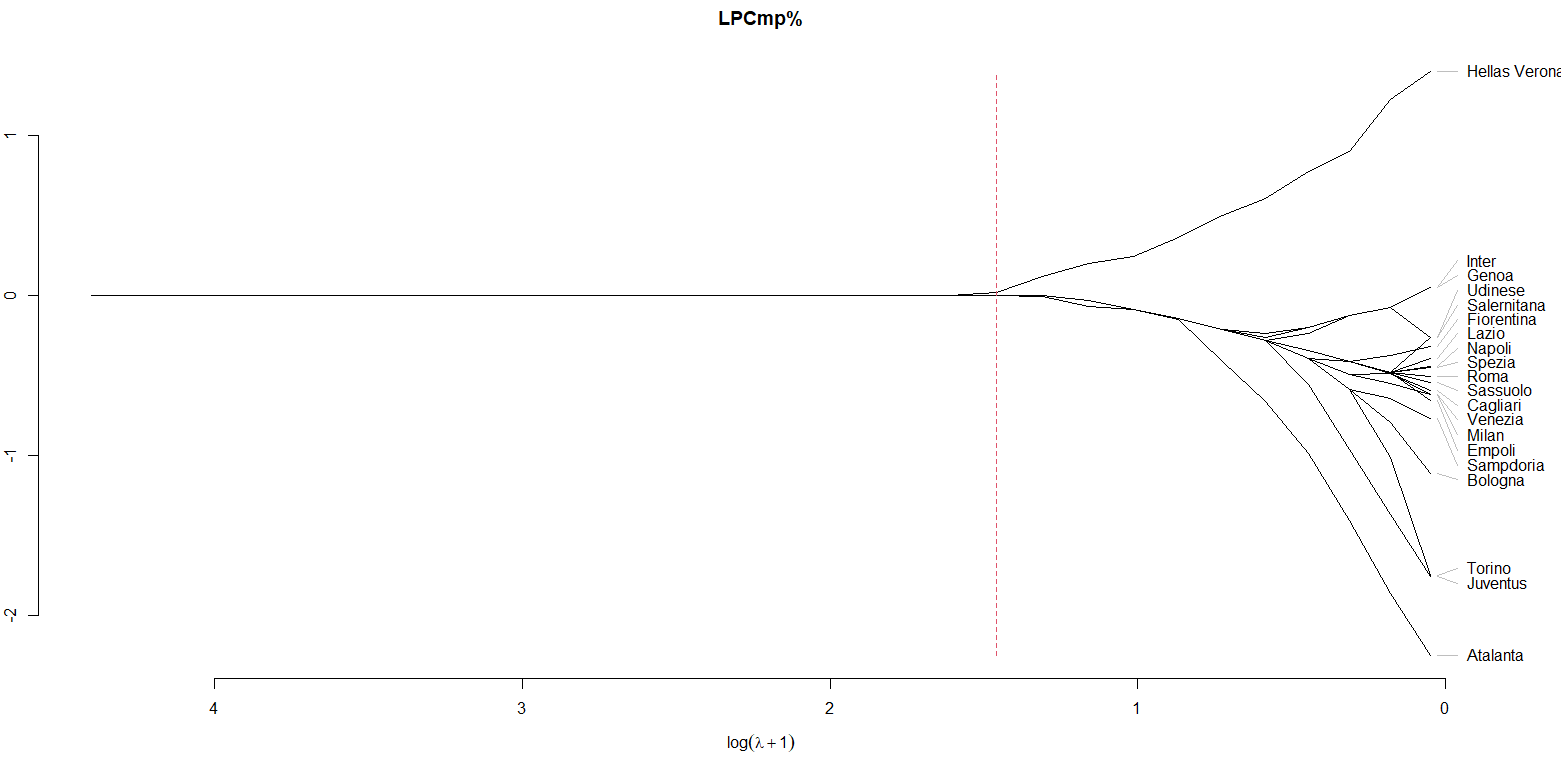
\includegraphics[height=8cm, width=15cm]{lpcmpLI.png}
		\caption{Grafico che riporta l'andamento della stima della percentuale di passaggi lunghi riusciti per ogni squadra al variare del parametro di tuning $\lambda$} \label{fig:lpcmpLI}
	\end{center}
\end{figure}
Sia il numero di tocchi fatti in area di rigore \texttt{ToDefPen} e sia il numero di tocchi fatti nella trequarti di difesa \texttt{ToDef3rd} aumentano la probabilità di vittoria. Nella stima del parametro della covariata che indica il numero di tocchi fatti a centrocampo \texttt{ToMid3rd}, viene a crearsi un cluster con un percorso quasi nullo contenente quasi tutte le squadre eccetto l'Inter e la Sampdoria, le quali formano un cluster con un percorso nullo.\\
Il numero di tocchi fatti nella trequarti offensiva \texttt{ToAtt3rd} è ancora stimato con un peso che diminuisce la probabilità di vittoria.\\
Per la stima della variabile esplicativa che indica il numero di tocchi fatti nell'area di rigore avversaria \texttt{ToAttPen}, c'è un cluster con un percorso negativo contenente quasi tutte le squadre eccetto l'Atalanta che si distingue con un percorso positivo. Tali risultati sono visibili nella Figura \ref{fig:toattpenLI}.\\
\begin{figure}[htbp]
	\begin{center}
		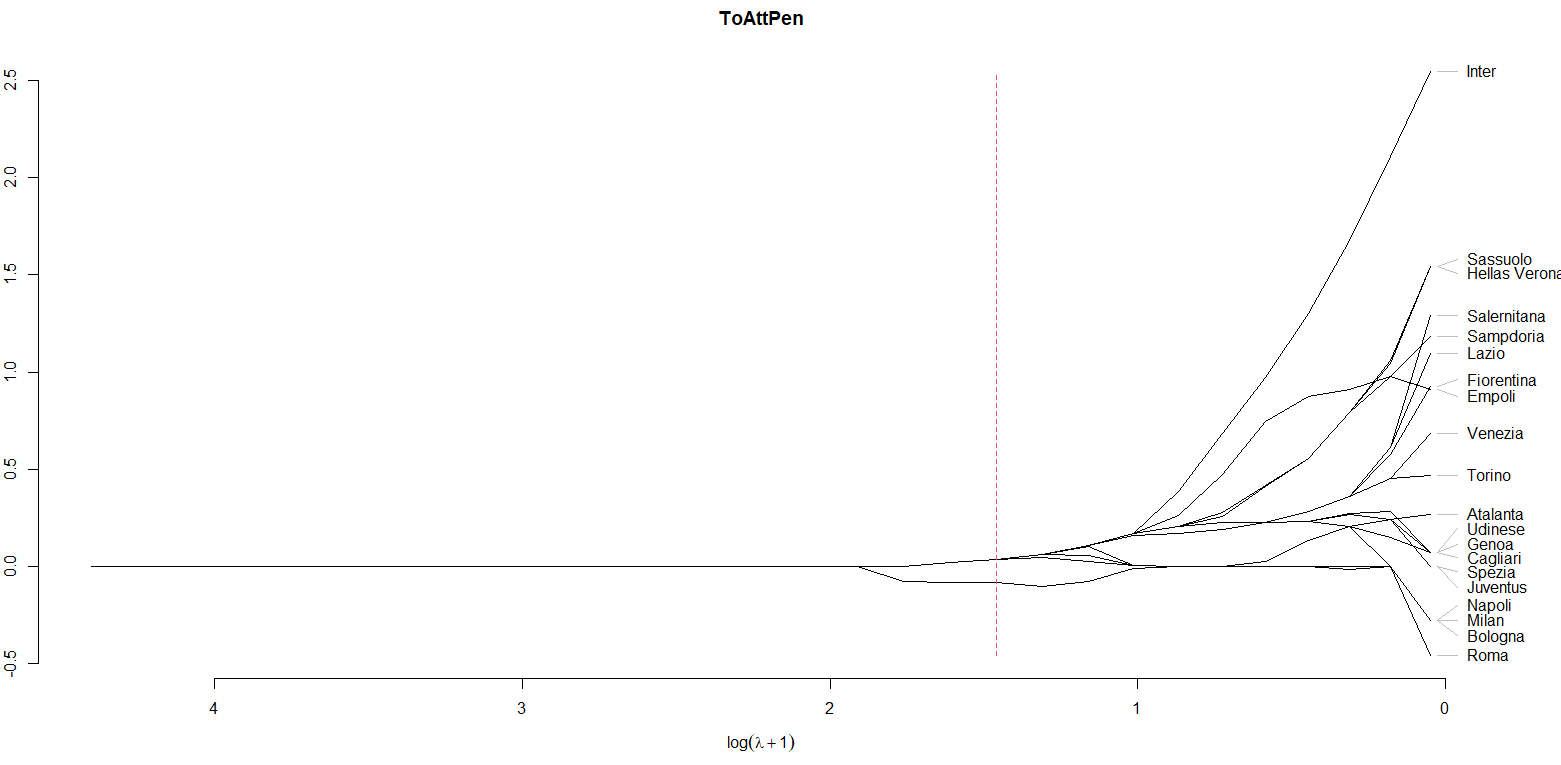
\includegraphics[height=8cm, width=15cm]{toattpenLI.png}
		\caption{Grafico che riporta l'andamento della stima del numero di tocchi fatti nell'area di rigore avversaria per ogni squadra al variare del parametro di tuning $\lambda$} \label{fig:toattpenLI}
	\end{center}
\end{figure}
Per quanto riguarda l'aggressività della squadra il numero di falli fatti \texttt{Fld} aumenta la probabilità di vittoria per tutte le squadre. Come mostrato della Figura \ref{fig:fldLI} però, la stima per l'Udinese è minore rispetto a tutte le altre squadre. Analogamente anche il numero di falli subiti \texttt{Fls} aumenta la probabilità di vittoria di tutte le squadre, in particolare il Bologna si distingue con una stima maggiore come mostrato nella Figura \ref{fig:flsLI}.\\
\begin{figure}[]
	\begin{center}
		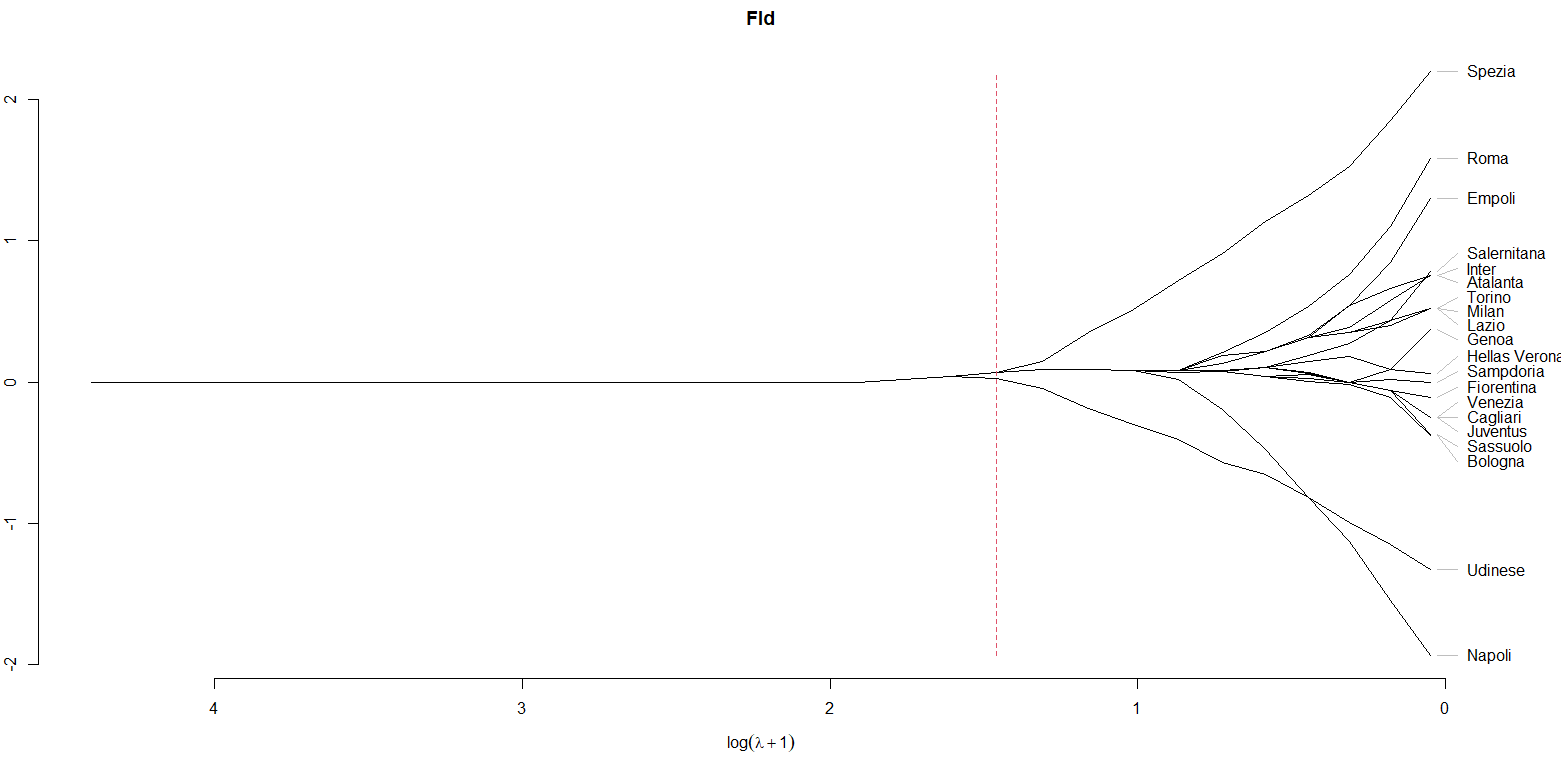
\includegraphics[height=8cm, width=15cm]{fldLI.png}
		\caption{Grafico che riporta l'andamento della stima del numero di falli fatti per ogni squadra al variare del parametro di tuning $\lambda$} \label{fig:fldLI}
	\end{center}
\end{figure}
\begin{figure}[htbp]
	\begin{center}
		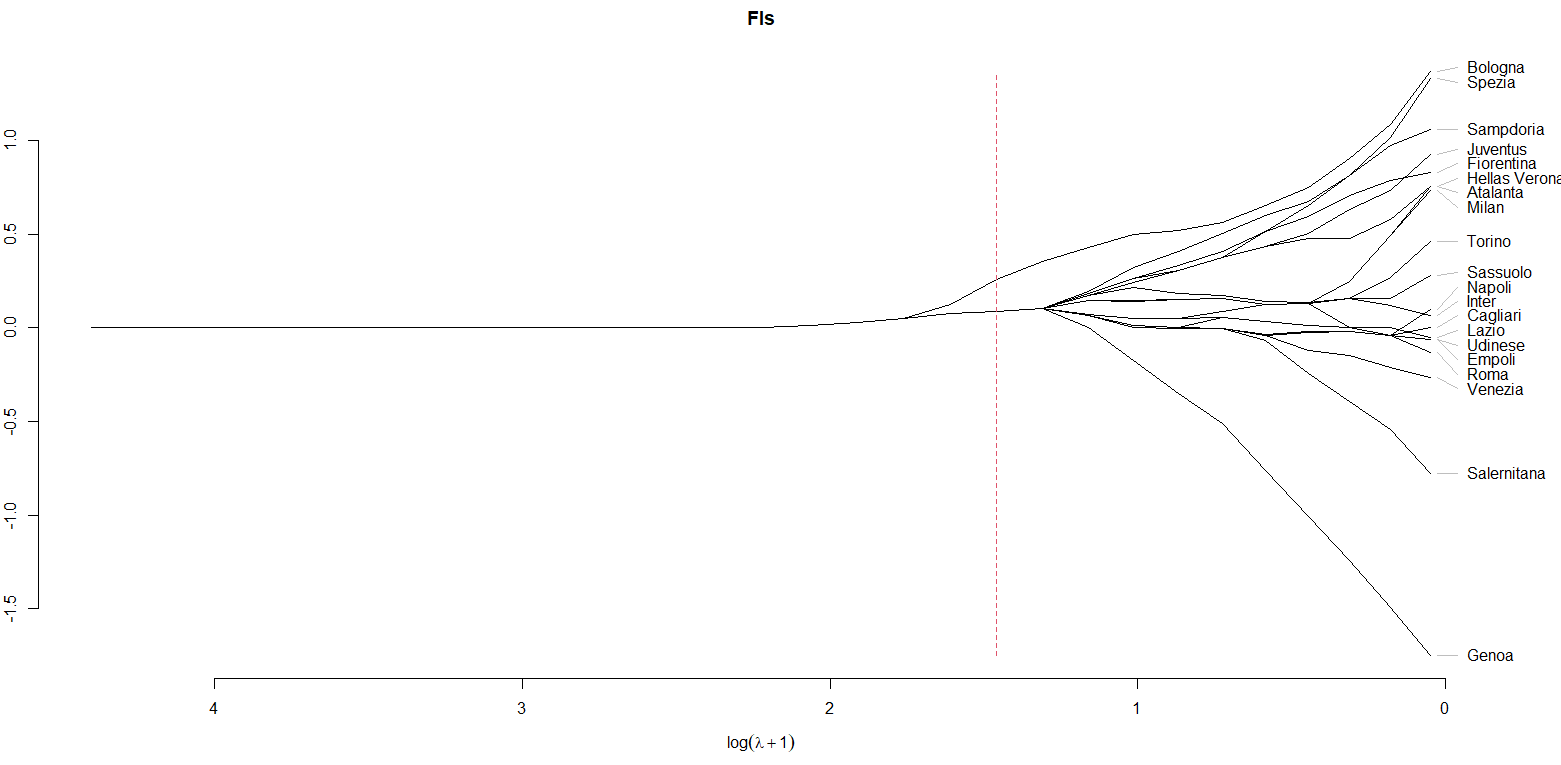
\includegraphics[height=8cm, width=15cm]{flsLI.png}
		\caption{Grafico che riporta l'andamento della stima del numero di falli subiti per ogni squadra al variare del parametro di tuning $\lambda$} \label{fig:flsLI}
	\end{center}
\end{figure}

Nella stima della covariata che indica il numero di fuorigioco fatti \texttt{Off}, viene a crearsi un cluster con un percorso nullo contenente quasi tutte le squadre eccetto la Juventus, la quale forma un cluster con un percorso negativo, tali risultati sono visibili nella Figura \ref{fig:offLI}.\\
\begin{figure}[htbp]
	\begin{center}
		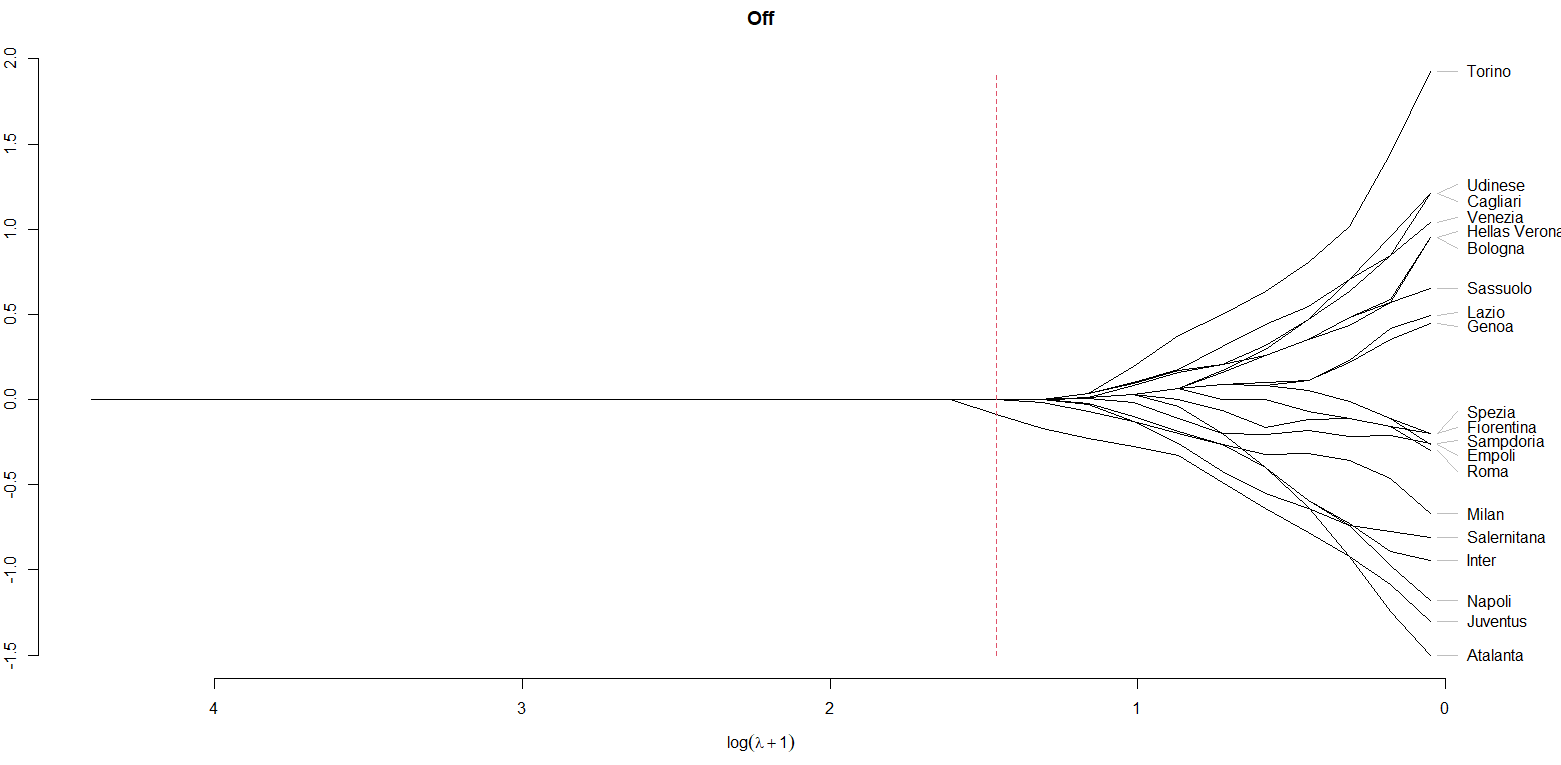
\includegraphics[height=8cm, width=15cm]{offLI.png}
		\caption{Grafico che riporta l'andamento della stima del numero di fuorigioco fatti per ogni squadra al variare del parametro di tuning $\lambda$} \label{fig:offLI}
	\end{center}
\end{figure}
La stima della variabile esplicativa del numero di cross fatti \texttt{Crs} si conferma essere ancora determinante per diminuire la probabilità di vittoria. L'Atalanta inoltre si distingue dalle altre squadre con un percorso ancora pù negativo rispetto, come mostrato nella Figura \ref{fig:crsLI}.\\
\begin{figure}[htbp]
	\begin{center}
		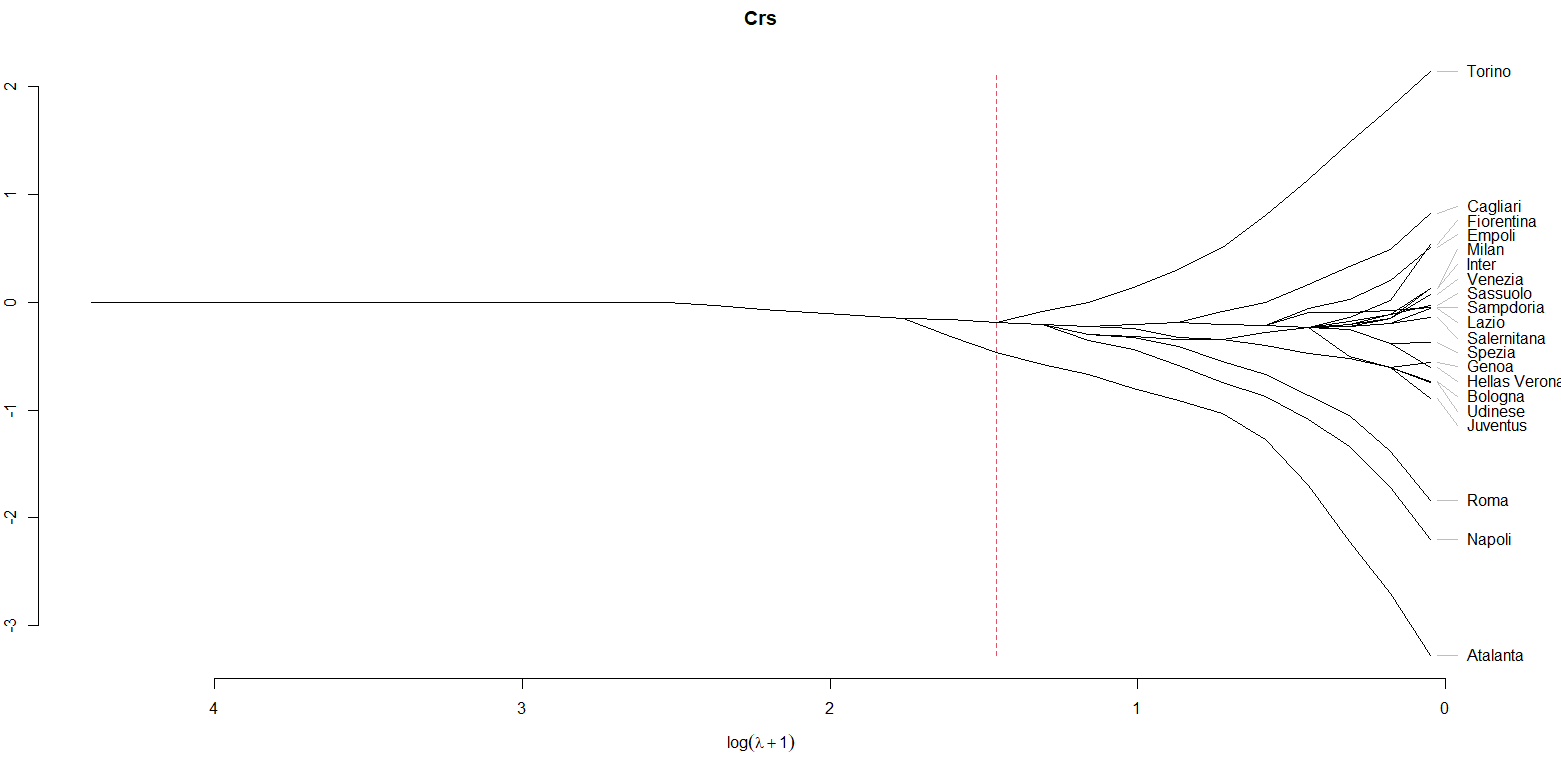
\includegraphics[height=8cm, width=15cm]{crsLI.png}
		\caption{Grafico che riporta l'andamento della stima del numero di cross fatti per ogni squadra al variare del parametro di tuning $\lambda$} \label{fig:crsLI}
	\end{center}
\end{figure}
Si nota che nella stima della covariata che indica il numero di contrasti vinti \texttt{TklWin}, viene a crearsi un cluster con un percorso nullo contenente quasi tutte le squadre eccetto l'Empoli, il quale forma un cluster con un percorso positivo. Tali risultati sono visibili nella Figura \ref{fig:tklwinLI}.\\
\begin{figure}[htbp]
	\begin{center}
		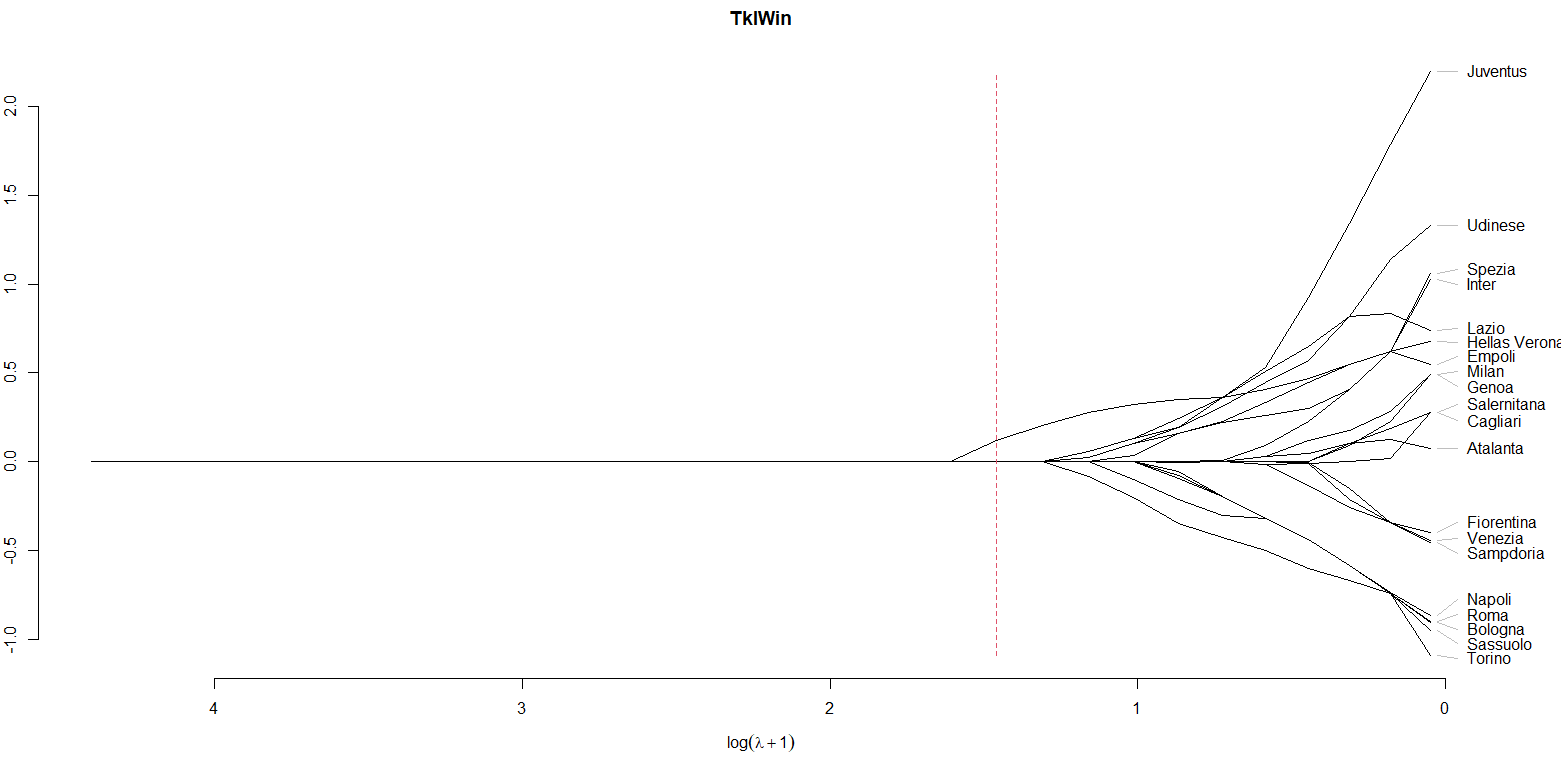
\includegraphics[height=8cm, width=15cm]{tklwinLI.png}
		\caption{Grafico che riporta l'andamento della stima del numero di contrasti vinti per ogni squadra al variare del parametro di tuning $\lambda$} \label{fig:tklwinLI}
	\end{center}
\end{figure}
Infine, viene confermato che giocare la partita \texttt{Home} ha un effetto positivo stimato in 0.270, mentre è cambiato la stima delle soglie $\theta_1$ e $\theta_2$ che valgono rispettivamente -0.803  e 0.803 .\\
Tutti i risultati sono stati ottenuti impostando come parametro di tuning $lambda$ pari a 3.299.\\

Un ulteriore analisi che può essere condotta, è analizzare l'effetto medio dei valori assunti per ogni partita e per ogni squadra delle covariate, insieme alle stime dei singoli parametri per squadra. Si utilizzeranno i grafici a \emph{effetto stella} proposti da \textcite{tutz2013visualization}. In questi grafici è possibile visualizzare i valori medi per squadra e per covariata moltiplicati per le rispettive stime riportate precedentemente. Quindi verrà illustrato graficamente il contributo medio di una variabile esplicativa sull'abilità di una singola squadra. Il grafico funziona nel seguente modo: esso mostra il prodotto esponenziale tra la media dei valori assunti da una covariate e le sue stime per ogni squadra. Per ogni grafico, viene creato un cerchio con raggio \emph{exp(0) = 1} il quale rappresenta il caso con stima nulla. I valori oltre il cerchio indica che la covariata ha effetto positivo in media sulla squadra, viceversa, i valori all'interno del cerchio indicano che la variabile esplicativa applica effetti negativi in media sulla squadra. Nella Figura \ref{fig:effstar1} nella Figura \ref{fig:effstar2} e nella Figura \ref{fig:effstar3} vengono mostrati i grafici a \emph{effetto stella}.
Nella Figura \ref{fig:effstar1} si possono vedere tutte le variabili esplicative con una stima nulla ma anche quelle covariate dove c'erano alcune squadre che si differenziavano dalle altre con una stima differente da quella nulla. Ad esempio la Lazio con il possesso palla \texttt{Poss} e l'Empoli con il numero di contrasti vinti \texttt{TklWin}.\\

\begin{figure}[htbp]
	\begin{center}
		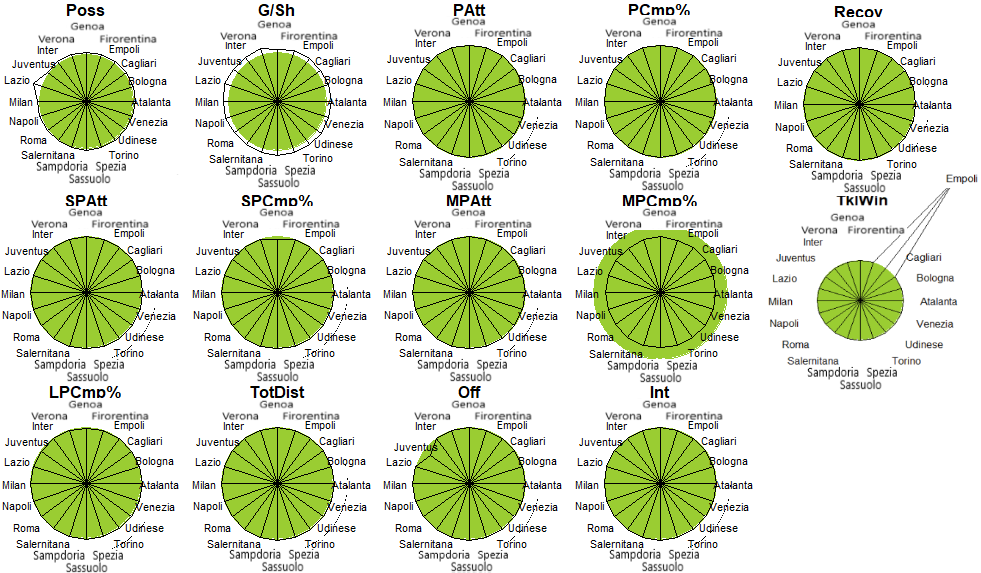
\includegraphics[height=9cm, width=15cm]{effstar.png}
		\caption{Grafico che riporta il contributo medio di una covariata sull'abilità di una singola squadra secondo il modello \ref{for:5.2}.} \label{fig:effstar1}
	\end{center}
\end{figure}

Per la Figura \ref{fig:effstar2} abbiamo due particolari grafici. Entrambi rappresentano l'effetto negativo delle covariate che indicano rispettivamente, il numero di tocchi nella trequarti avversaria fatti \texttt{ToAtt3rd} e il numero di cross fatti \texttt{Crs}. In particolare notiamo che a subire più gli effetti negativi sono l'Inter e l'Atalanta in entrambe le variabili esplicative. 


\begin{figure}[htbp]
	\begin{center}
		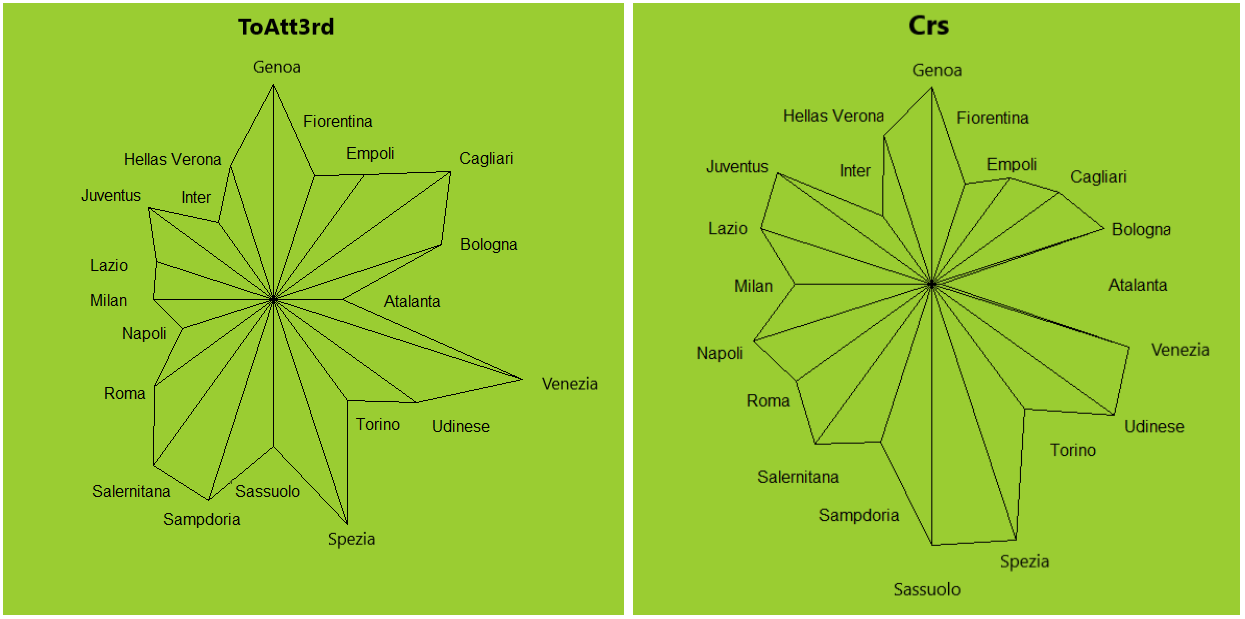
\includegraphics[scale = 0.40]{estarL2.png}
		\caption{Grafico che riporta il contributo medio di una covariata sull'abilità di una singola squadra secondo il modello \ref{for:5.2}.} \label{fig:effstar2}
	\end{center}
\end{figure}

Infine, risultati più interessanti si hanno nella Figura \ref{fig:effstar3}. Innanzitutto si vede che nella nel grafico del numero di tiri \texttt{Sh} l'Inter ha un grosso beneficio, ma anche in minor misura il Milan, la Roma, l'Atalanta, il Napoli, la Juventus e il Sassuolo. Perciò in generale come già visto \texttt{Sh} ha un effetto positivo e ancora di più per le squadre elencate. Analoghi risultati sono visibili con il numero di tiri in porta \texttt{SoT} con l'aggiunta della Lazio tra le squadre che ricevano più benefici. In generale, nel grafico del numero di parate \texttt{Saves} tutte le squadre ottengo benefici, stesso risultato ma più importante anche con il numero di passaggi lunghi tentati \texttt{LPAtt}. Nel grafico del numero di tocchi in area di rigore \texttt{ToDefPen} c'è un particolare beneficio ottenuto dal Venezia ma anche dell'Inter, dalla Lazio, dall'Empoli e dal Sassuolo. Analoghi risultati anche per il numero di tocchi nella trequarti difensiva \texttt{ToDef3rd}, ma con la differenza di minori benefici per il Venezia. Pertanto, si nota la tendenza delle squadre italiana a attuare tattiche che prediligono di giocare nella propria metà campo. Il numero di tocchi a centrocampo \texttt{ToMid3rd} vengono in media effettuati molto dalle squadre, tranne per le eccezioni Inter e Sampdoria dove l'effetto è nullo. Analogo effetto anche per il numero di tocchi fatti in area di rigore \texttt{ToAttPen}, con l'unica differenza che ora Inter e Sampdoria hanno un effetto positivo e solo l'Atalanta ha un effetto negativo. In generali i falli subiti \texttt{Fls} portano benefici alle squadre sopratutto al Bologna come si era notato dalle stime del modello. Per i falli fatti invece abbiamo che l'Udinese ha minor benefici rispetto a tutte le altri squadre come visto nelle stime.\\
\begin{figure}[htbp]
	\begin{center}
		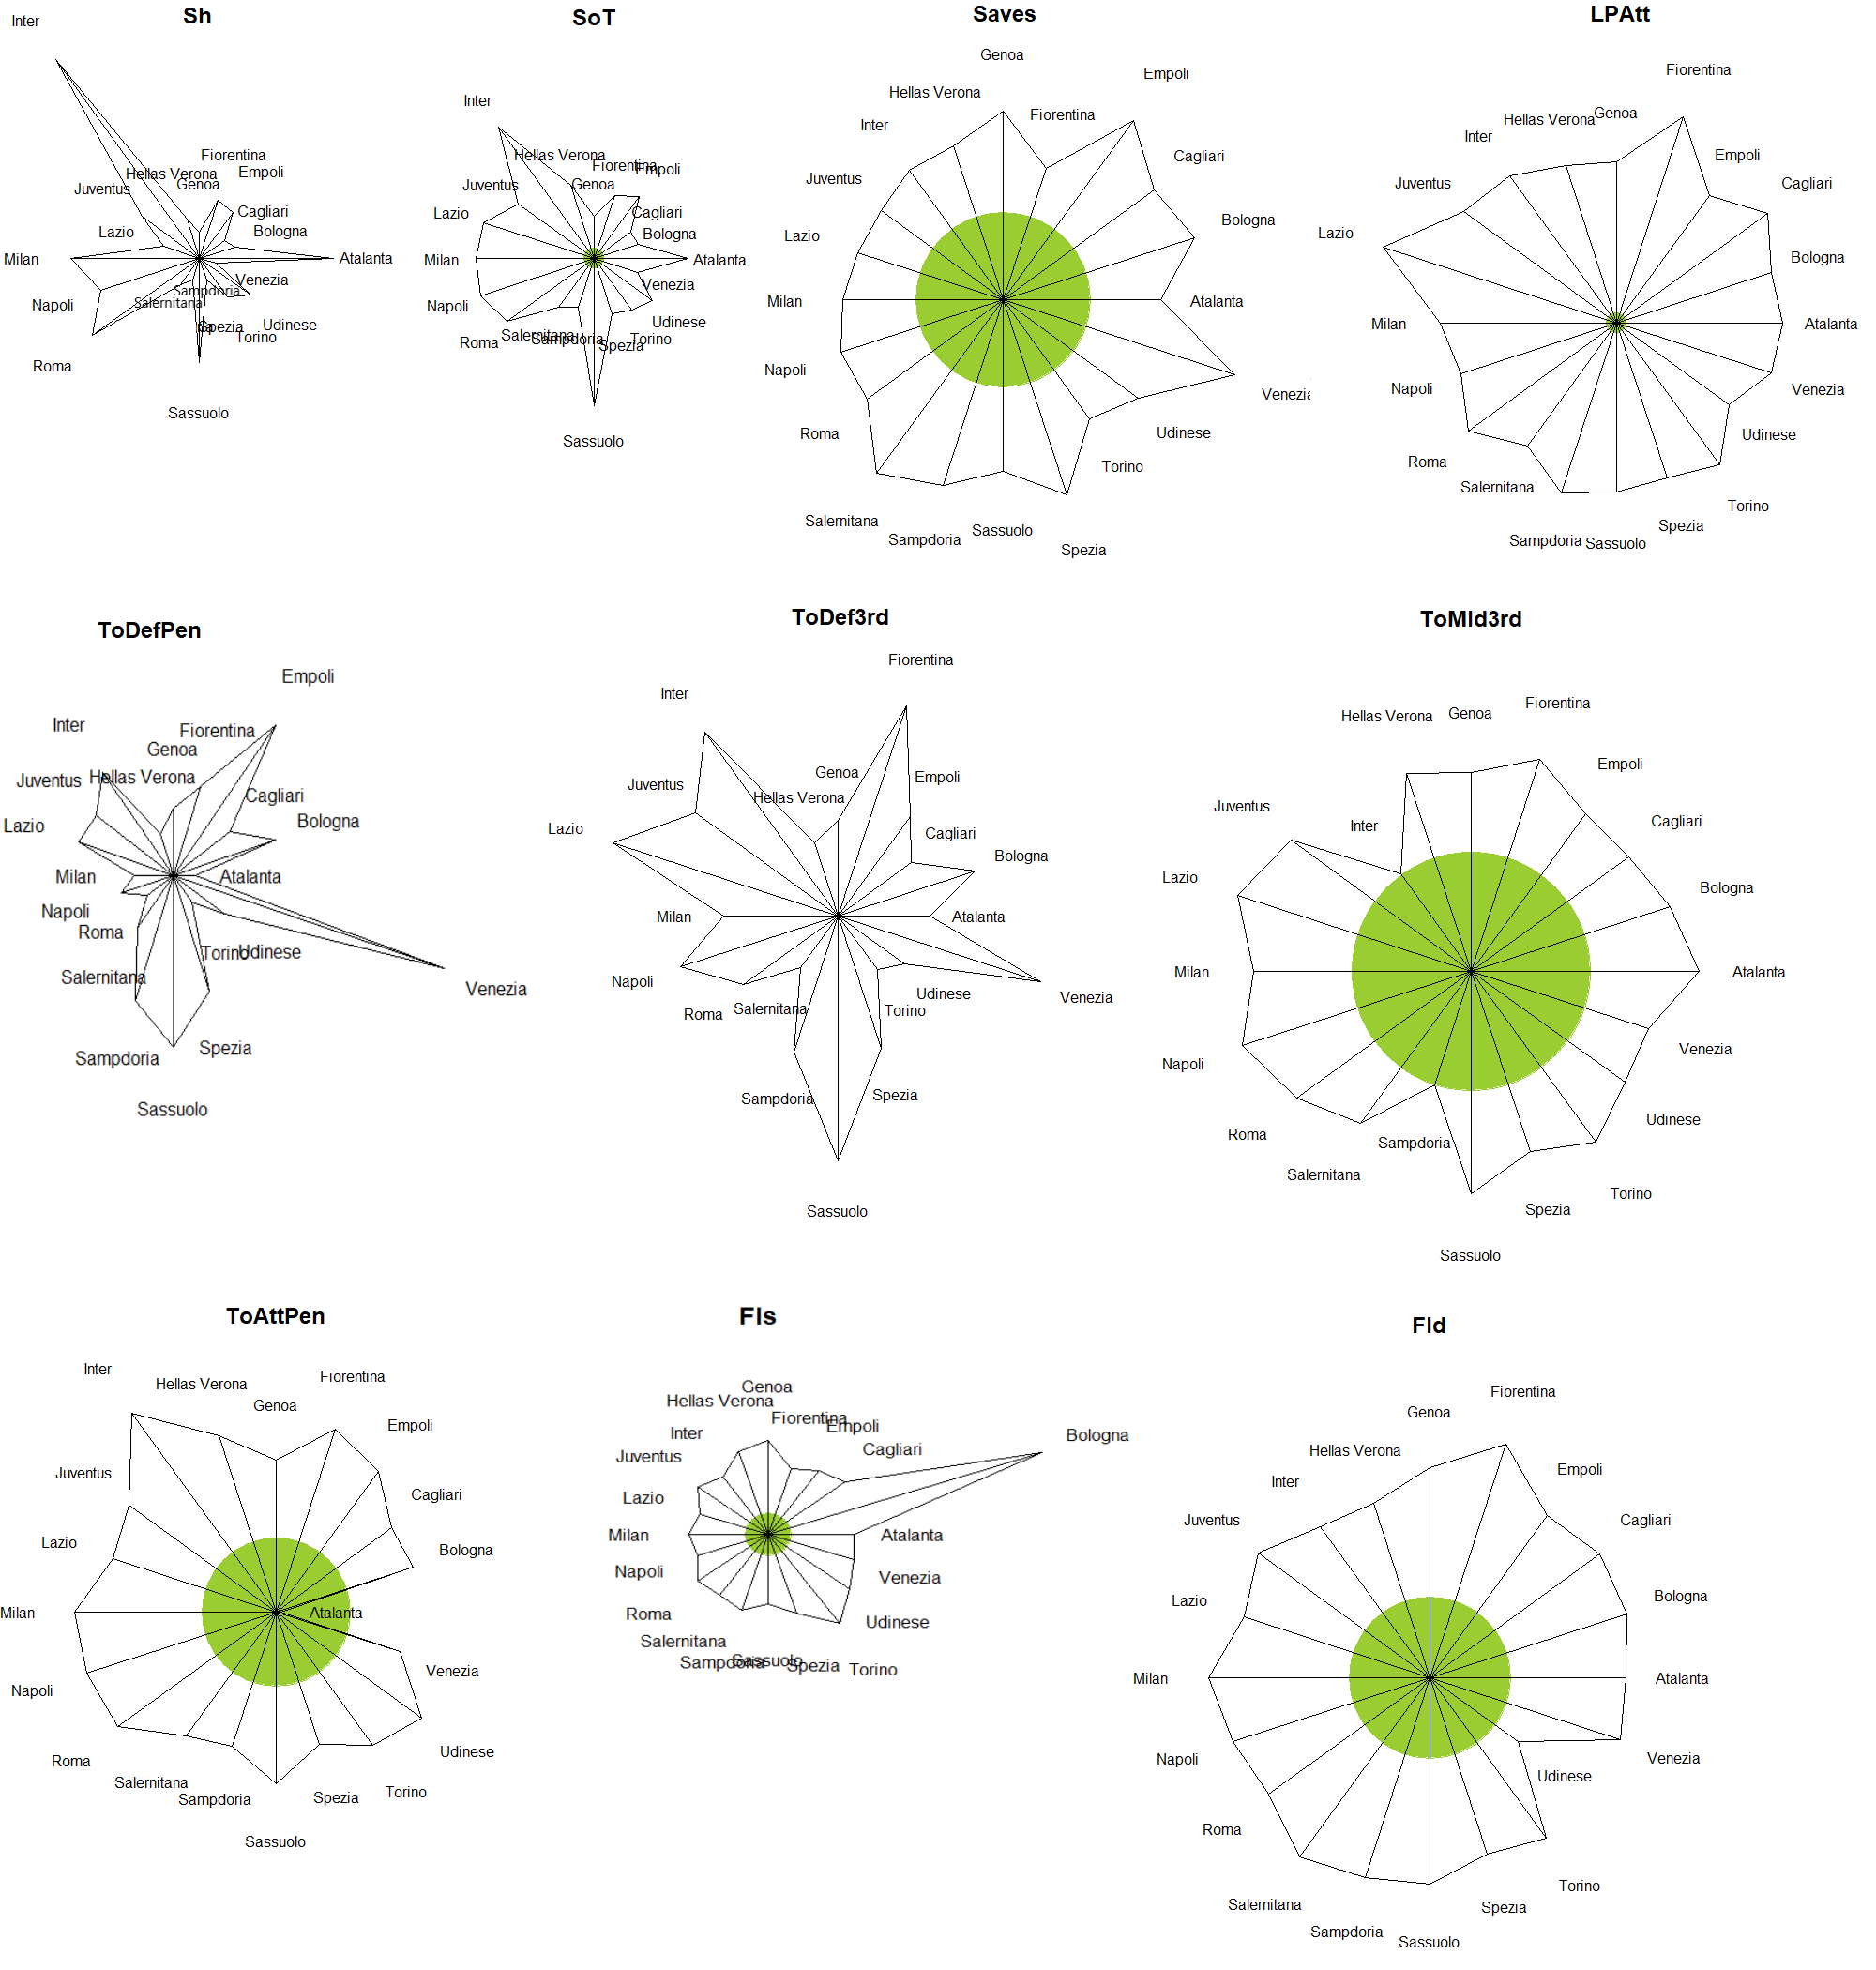
\includegraphics[height=16cm, width=16cm]{estarL.png}
		\caption{Grafico che riporta il contributo medio di una covariata sull'abilità di una singola squadra secondo il modello \ref{for:5.2}.} \label{fig:effstar3}
	\end{center}
\end{figure}

Infine come fatto nella sezione precedente, si analizzano i percorsi delle norme L2 che rappresentano l'importanza complessiva dei singoli effetti delle covariate. Tali percorsi sono visibili nella Figura \ref{fig:IL2}.

\begin{figure}[htbp]
	\begin{center}
		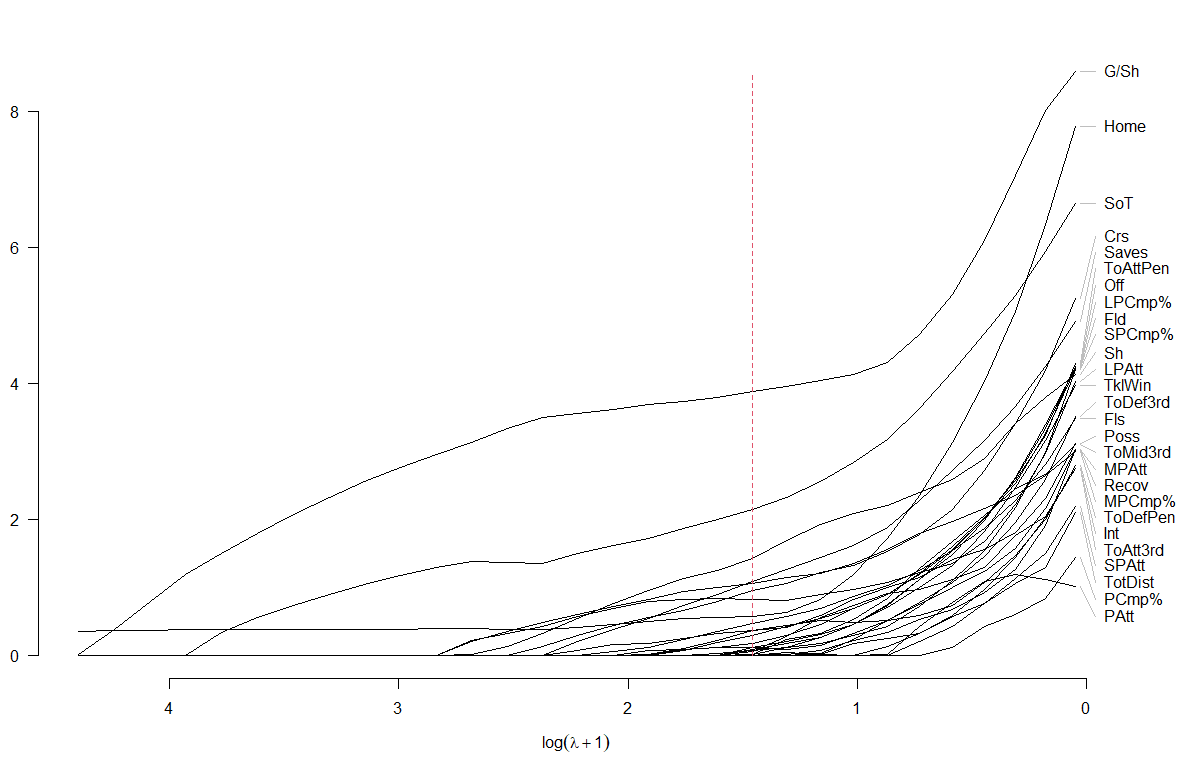
\includegraphics[height=8cm, width=15cm]{IL2.png}
		\caption{Grafico che riporta l'importanza delle covariate rispetto alle norme L2 al variare del parametro di tuning $\lambda$} \label{fig:IL2}
	\end{center}
\end{figure}

Gli andamenti ottenuti nella Figura \ref{fig:IL2} sono molto simili a quelli visti nella Figura \ref{fig:l2BTCL}, con però un aumento di importanza per la covariata \texttt{ToAttPen} in termini di diminuzione della probabilità di vittoria. Pertanto, quanto ricavato del modello (\ref{for:4.9}) ora trova conferma anche nel modello (\ref{for:5.2}).\\

\section{Conclusione dei risultati ottenuti}(BOZZA)
(*****Probabilmente da spostare nel capitolo delle conclusioni*****)\\

Dai risultati ottenuti e dalle analisi condotte è possibile affermare la seguente conclusione. Nel campionato italiano per poter vincere o comunque ottenere dei buoni risultati la squadra deve adottare un comportamento tattico e giocare prevalentemente nella propria metà campo. Quindi, un comportamento meno propenso a controllare il pallone per lungo tempo, infatti abbiamo il possesso della palla \texttt{Poss} e la distanza percorsa con la palla \texttt{TotDist} che non danno ne benefici ne svantaggi; ma più propenso a giocare maggiormente la palla nella propria area di difesa per evitare contropiedi, infatti le stime del numero di tocchi in area di rigore \texttt{ToDefPen}, il numero di tocchi nella trequarti difensiva \texttt{ToDef3rd} e il numero di tocchi a centrocampo \texttt{ToMid3rd} segnalano dei aumenti per la probabilità di vittoria. Avere perciò una buona difesa è fondamentale, infatti la stima dell'effetto del numero di parate \texttt{Saves} aumenta le probabilità di vittoria. La fase offensiva non deve essere troppo lunga in termini di possesso della palla, infatti il numero di tocchi fatti nella trequarti offensiva \texttt{ToAtt3rd} porta ad avere una diminuzione delle probabilità di vittoria ma se si fanno i giusti passaggi per entrare nell'area di rigore avversaria mantenendo sempre un possesso palla breve si aumentano le probabilità di vittoria come visto nella stima del numero di tocchi in area di rigore avversaria \texttt{ToAttPen}. Dalle analisi emerge che uno sbilanciamento verso la fase offensiva porta una forte diminuzione alle probabilità di vittoria. Infatti guardando i casi di Inter e Atalanta abbiamo che: l'Inter da i dati si dimostra essere una dalle squadre che più tira in generale \texttt{Sh} e in porta \texttt{SoT}, analogamente anche l'Atalanta. Entrambe però mantengo troppo il controllo del pallone nell'area avversaria. Infatti per entrambe le squadre ci sono pesanti diminuzioni della probabilità di vittoria a causa della stima del parametro di \texttt{ToAtt3rd}. Peggio ancora per l'Atalanta, che ha un gioco particolarmente offensivo (vedi \textit{\cite{ataGioco}}), che le fa ottenere una diminuzione della probabilità della vittoria dalla stima del parametro \texttt{ToAttPen}. Questo perché il prolungato controllo del pallone la porta l'Atalanta a esporsi e a subire contropiedi. Si è parlato spesso di contropiedi nella nostra analisi, infatti quello che emerge sempre in tema di fase offensiva è che, il numero di tiri è relativamente basso e questo lo si capisce dal fatto c'è un enorme aumento della probabilità di vittoria portato della stima del rapporto tiri-gol \texttt{G/Sh}. Quello che si vuole intendere è che le squadre attaccano poco e quando attaccano cercano di massimizzare la loro fase offensiva, infatti le partite nel campionato italiano spesso finiscono con al massimo due o tre gol segnati in totale. Pertanto, l'efficacia di un azione offensiva che porta al gol e la carenza di azioni offensive portano \texttt{Sh}, \texttt{SoT} ma soprattutto \texttt{G/Sh} ad assumere un elevato peso nel determinare la vittoria. Concludendo la trattazione sulla fase offensiva, si illustra qual'è il miglior modo di attaccare che emerge dai modelli. Si sa che il contropiede è efficace ma allo stesso tempo difficile da attuare per via del comportamento delle squadre a non sbilanciarsi. Una valida alternativa che emerge è il lancio lungo che parte dall'area che va dall'area di rigore della squadra fino a centrocampo, ed arriva nell'area avversaria. Infatti la stima del parametro del numero di passaggi lunghi tentati \texttt{LPAtt} aumenta la probabilità di vittoria. L'utilizzo di passaggi filtrati non è una buona tattica, infatti la stima del parametro \texttt{MPCmp\%} diminuisce la probabilità di vittoria. Analogamente anche i cross \texttt{Crs} non danno benefici ma anzi svantaggi, infatti ancora una volta ne rimangono penalizzate l'Inter e soprattutto l'Atalanta che con il suo gioco sfrutta molto le fasce (vedi \textit{\cite{ataGioco}}). Concludendo, è importante sottolineare che un atteggiamento da parte della squadra troppo speculativo o difensivo non porta alla vittoria. Questo è il caso del Venezia classificatosi come ultimo e che ha ottenuto gli effetti più alti dalle covariate \texttt{ToDefPen} e \texttt{ToDef3rd} ma bassi benefici dalle variabili esplicative offensive.

\section{Predizioni}
In questa sezione si vuole valutare le prestazione dei quattro modelli presentati. I modelli saranno valutati tra loro in base alle predizioni che hanno prodotto ciascuno. Per predizione si intende che il modello stabilisce l'esito di una partita senza conoscerne il risultato reale. Per rendere più interessante il confronto si aggiungere un quinto elemento nel confronto, ossia le predizioni fatte dai \emph{bookmakers}, ad esempio Bet365, William Hill ecc.. I dati dei \emph{bookmakers} sono stati presi da \textit{\cite{bet}}, il quale fornisce la media delle probabilità dei \emph{bookmakers} per ogni risultato, su un gran numero di campionati di calcio tra cui la Serie A italiana. Si è quindi preso come predizione il risultato più probabile secondo i \emph{bookmakers}.\\
Le predizioni dei modelli sono state eseguite nel seguente modo: il \emph{dataset} è stato diviso in modo casuale in due parti chiamate solitamente \emph{training set} e \emph{test set}. Il \emph{training set} contiene quasi l'80\% delle 38 giornate, ossia 30 giornate per un totale di 300 partite. Invece il \emph{test set} contiene circa il restante 20\% ossia 8 giornate per un totale di 80 partite. Il \emph{training set} è utilizzato per stimare i parametri del modello mentre il \emph{test set} è utilizzato per fare predizione. Perciò una parte delle osservazione sono state utilizzate per allenare il modello, mentre la restante parte per predire l'esito delle restanti osservazioni. \\
Prima di discutere delle misurazioni e delle predizioni ottenute, è importante tener presente che, i modelli (\ref{for:3.1}), (\ref{for:5.1}), (\ref{for:4.9}) e (\ref{for:5.2}), utilizzano informazioni e statistiche che sono disponibili solo dopo il termine delle partite, cioè non disponibili per i \emph{bookmakers}. Infatti i \emph{bookmakers} calcolano le loro predizioni prima che le partite comincino ma tenendo conto delle informazione delle partite precedentemente giocate. Certamente i quattro modelli non sono utilizzabili per poter fare predizioni, ma l'obbiettivo del confronto è quello di capire se le informazioni sono state impiegate in modo ragionevole per acquisire maggior conoscenza. Ciò è possibile notarlo se i modelli hanno prestazioni superiori alle predizioni dei \emph{bookmakers}.\\
Le metriche che saranno usate per valutare le predizione calcolate sono le seguenti:
\begin{itemize}
	\item \texttt{Accuratezza}. Indica il rapporto tra il numero di predizioni classificate correttamente e il numero totale delle osservazioni in esame.
	\item \texttt{Sensibilità}. Indica il rapporto tra il numero di predizioni identificate correttamente con la categoria \emph{k} e il numero totale delle osservazioni classificate con la categoria \emph{k} con \emph{k $\in$ \{1,....,K\}}.
	\item \texttt{Specificità}. Indica il rapporto tra il numero di predizioni identificate correttamente con una categoria diversa dalla categoria \emph{k} e il numero totale delle osservazioni classificate con una categoria diversa dalla categoria \emph{k} con \emph{k $\in$ \{1,....,K\}}.
\end{itemize}
Nella Figura \ref{fig:pre} sono mostrate le classificazione ottenute sulle 80 partite del \emph{test set} per ogni modello e per la predizione dei \emph{bookmakers}.
\begin{figure}[htbp]
	\begin{center}
		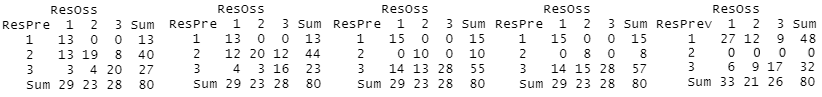
\includegraphics[scale = 0.60]{tabpre.png}
		\caption{La prima tabella indica le predizioni di 80 partite fatte dal modello (\ref{for:3.1}), la seconda dal modello (\ref{for:5.1}), la terza dal modello (\ref{for:4.9}), la quarta dal modello (\ref{for:5.2}) e la quinta dai \emph{bookmakers}
			\label{fig:pre}}
	\end{center}
\end{figure}
%36 sbagliate 55%

Dai risultati ottenuti, l'accuratezza dei quattro modelli è rispettivamente 0.65, 0.6125, 0.6625 e 0.6375, mentre per i \emph{bookmakers} è di 0.55. Si può subito notare che tutti e quattro i modelli sono migliori delle predizioni dei \emph{bookmakers}. In particolare il modello (\ref{for:4.9}) risulta essere quello che produce più predizioni corrette. Sorprendentemente il modello (\ref{for:3.1}) che utilizza solo le abilità medie delle squadre e quindi senza l'utilizzo delle variabili esplicative risulta essere migliore di tutti eccetto per il modello (\ref{for:4.9}). In particolare si conferma quanto enunciato nel Capitolo \ref{cap:BT} riguardo al ruolo dell'intercetta e delle covariate, infatti il modello senza intercetta (\ref{for:5.2}) risulta essere leggermente peggiore del modello con l'intercetta (\ref{for:4.9}). A tal proposito si può confermare l'esistenza di una differente relazione delle variabili esplicative da squadra a squadra. Infatti tra i quattro modelli confrontati, il modello (\ref{for:5.1}) ottiene le peggiori prestazioni dato che ha ignorato la diversa relazione delle variabili esplicative con ogni singola squadra.\\
Nella Figura \ref{fig:recall} vengono mostrate le misurazioni della sensibilità per ognuna delle delle tre categorie per i quattro modelli e per i \emph{bookmakers}.\\

\begin{figure}[htbp]
	\begin{center}
		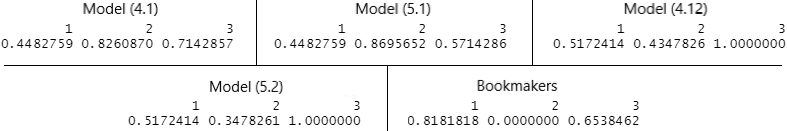
\includegraphics[scale = 0.60]{recall.png}
		\caption{La prima tabella indica le sensibilità delle predizioni del modello (\ref{for:3.1}), la seconda del modello (\ref{for:5.1}), la terza del modello (\ref{for:4.9}), la quarta del modello (\ref{for:5.2}) e la quinta dei \emph{bookmakers}
			\label{fig:recall}}
	\end{center}
\end{figure}
Come si può notare i \emph{bookmakers} hanno molti problemi a classificare correttamente l'esito di una partita quando questa termina con un pareggio. Infatti vediamo che la sensibilità è zero, questo perché ci sono zero partite classificate con il pareggio, ma dai dati osservati si sa che ci sono delle partite che terminano con un pareggio. Tuttavia sono molto affidabili nel predire la vittoria della squadra in casa contro la squadra ospite. I modelli (\ref{for:4.9}) e (\ref{for:5.2}) sanno classificare correttamente quando la squadra ospite batte la squadra in casa, infatti la sensibilità è a uno, il massimo. Infine notiamo che i modelli (\ref{for:3.1}) e (\ref{for:5.1}) sanno ben identificare una partita che termina con un pareggio.\\
Nella Figura \ref{fig:speci} vengono mostrate le misurazioni della specificità per ognuna delle tre categorie per i quattro modelli e per i \emph{bookmakers}. \\
\pagebreak
\begin{figure}[htbp]
	\begin{center}
		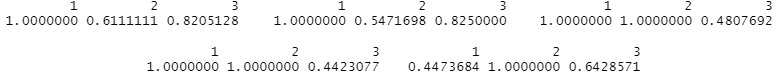
\includegraphics[scale = 0.60]{specificity.png}
		\caption{La prima tabella indica le specificità delle predizioni del modello (\ref{for:3.1}), la seconda del modello (\ref{for:5.1}), la terza del modello (\ref{for:4.9}), la quarta del modello (\ref{for:5.2}) e la quinta dei \emph{bookmakers}
			\label{fig:speci}}
	\end{center}
\end{figure}

Ovviamente in questa misurazione i \emph{bookmakes} ottengono il miglior risultato per quanto riguarda l'identificare se una partita non termina in un pareggio. Si nota che tutti e quattro i modelli sanno ben identificare quando l'esito della partita non è la vittoria della squadra di casa, infatti la misurazione ottenuta è uno. Inoltre anche i modelli (\ref{for:4.9}) e (\ref{for:5.2}) sanno ben identificare quando una partita non termina in un pareggio. D'altra parte i modelli (\ref{for:3.1}) e (\ref{for:5.1}) ottengono le migliori misurazione nell'identificare quando una partita non termina con la vittoria della squadra ospite.\\

In conclusione, dai risultati ottenuti si può affermare di aver utilizzato correttamente le informazioni a disposizione dato che si ottengono in generale, prestazioni migliori rispetto alle predizioni dei \emph{bookmakers}.